\documentclass[a4paper]{article}

\usepackage[T1]{fontenc}
\usepackage[spanish]{babel}

\usepackage{subfig,graphicx, geometry, array, booktabs, float, hyperref, setspace}

% Make text height 5% larger than the default
\setlength{\textheight}{1.05\textheight}

% Remove labels and center all captions
\captionsetup[subfigure]{labelformat=empty,justification=centering}
\captionsetup{justification=centering,margin=0.7cm,labelformat=empty}

% Include references on TOC
\usepackage[nottoc,numbib]{tocbibind}

\usepackage[dvipsnames]{xcolor}
\hypersetup{
    colorlinks=true,
    linkcolor=black,
    urlcolor=RoyalBlue,
    citecolor=black
}


\begin{document}

\begin{titlepage}
    \newgeometry{top=0.6in,bottom=0.6in,right=1in,left=1in}

    \centering
    \hfill
    \begin{minipage}{0.7\textwidth}
            \centering
            \LARGE
            \textsc{\textbf{Facultad de Ingeniería}}\\[0.1cm]
            \textsc{\textbf{Universidad de Buenos Aires}}
        \end{minipage}
        \begin{minipage}{2.6cm}
            \centering
            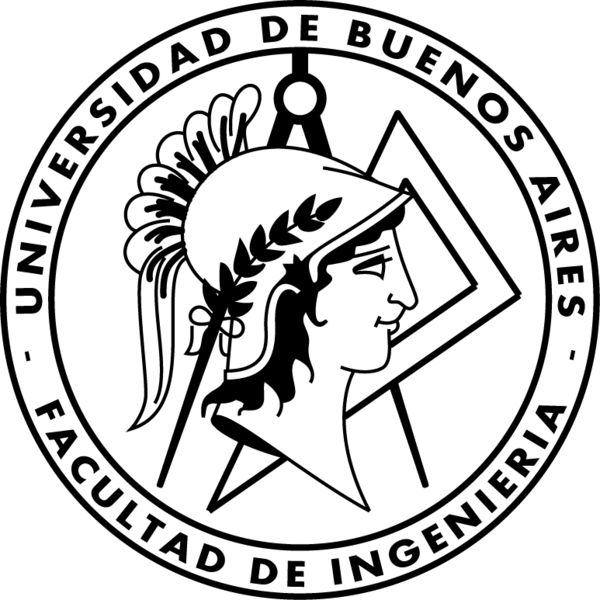
\includegraphics[width=2.6cm]{./img/fiuba.png}
        \end{minipage}

    \vspace{3cm}
    \huge \bfseries Trabajo Profesional \\
    \LARGE \bfseries Licenciatura en Análisis de Sistemas, Ingeniería en Informática
    \vspace{2cm}

    \rule{\linewidth}{0.3mm} \\[0.1cm]
    \huge \bfseries Sistema de detección en tiempo real de publicidad en la vía pública\\
    \vspace{0.1cm}
    \small\href{https://bart.fly.dev}{bart.fly.dev}
    \rule{\linewidth}{0.3mm}\\[0.7cm]

    \large \emph{Tutor:} Ing. Martín Buchwald\\[0.6cm]
    \begin{minipage}{0.4\textwidth}
        \begin{flushleft}
            \centering
            \large del Mazo, Federico \\
            100029
        \end{flushleft}
    \end{minipage}
    \begin{minipage}{0.4\textwidth}
        \begin{flushright}
            \centering
            \large Pastine, Casimiro \\
            100017
        \end{flushright}
    \end{minipage}
    \restoregeometry
\end{titlepage}

\tableofcontents
\newpage

\section{Motivación}

Dentro del marco de trabajo profesional de las carreras de Licenciatura en Análisis de Sistemas y de Ingeniería en Informática de la Facultad de Ingeniería, Universidad de Buenos Aires, se presenta el proyecto de un sistema de detección de publicidades en la vía pública en tiempo real.

La aspiración de este proyecto es presentar un \textit{software} que, a medida que un usuario graba un video, detecte si hay un cartel publicitario en algún cuadro del video, en qué porción del cuadro está, y devuelva este resultado de manera inmediata.

Durante la concepción de la idea del trabajo, nos planteamos los siguientes objetivos a alcanzar una vez concluído el desarrollo:

\begin{itemize}
    \item Aplicar los conocimientos interdisciplinarios de comprensión y evaluación de sistemas aprendidos en nuestra carrera académica en un campo enteramente nuevo para nosotros como lo es \textit{Computer Vision}.

    \item Realizar un proyecto integral con su debida investigación y comprensión del estado del arte en las disciplinas relevantes, abarcando desde el entrenamiento de un modelo de clasificación de objetos hasta el despliegue del sistema en algún entorno fácilmente accesible por el usuario final.

    \item Encontrarnos con desafíos prácticos como la falta de los datos necesarios para el modelo a entrenar y la evaluación y comparación de distintos métodos para lograr un rendimiento aceptable y encontrar las soluciones adecuadas para los obstáculos que vayan apareciendo, sopesando las distintas alternativas posibles que surgirán durante el desarrollo del trabajo.

    \item Lograr hacer un sistema de código abierto, modularizable y extensible tal que en un futuro se pueda cambiar cualquier eslabón de su cadena como los objetos a detectar, el algoritmo de detección y rastreo de objetos o el post procesamiento a aplicar.
\end{itemize}

El presente trabajo mostrará cómo se cumplieron estos objetivos a lo largo del camino de investigación y desarrollo que recorrimos.

\section{Descripción del Problema}

El núcleo de nuestro trabajo tiene una división lógica en dos problemas distintos.

Para comenzar, hablamos de \textbf{\textit{detectar} anuncios}. Lo que queremos decir con esto es que buscamos implementar un \textit{software} que, al mostrarle una imagen, nos sepa determinar exáctamente en qué parte de la misma se encuentra algo que consideramos como un anuncio, si es que este anuncio está presente.
Este tipo de problema cae bajo el campo de \textit{Computer Vision}, una rama de la inteligencia artificial que se dedica a comprender datos visuales y poder interpretar su contenido.

Por otro lado, buscamos hacer un sistema que funcione en \textbf{tiempo real}. Esto quiere decir que en vez de un \textit{software} que procese videos pre-grabados y le presente al usuario las detecciones después de haber solicitado el procesamiento, pretendemos que mientras el usuario apunte su cámara, pueda ver cuadro por cuadro cómo el sistema detecta los anuncios inmediatamente.
Esto nos presenta varios desafíos, principalmente enfocados en poder procesar cada cuadro en un tiempo razonable y aceptable para que el usuario pueda ver en su dispositivo lo que ve en la vida real sin una demora significativa.

\subsection{\textit{Computer Vision}}

El campo de \textit{Computer Vision} se refiere a la disciplina de la inteligencia artificial, específicamente en la rama de \textit{Machine Learning}, que se ocupa de permitir a las computadoras \textit{``ver''} y comprender el mundo visual de la misma manera que lo hacen los seres humanos. Utiliza diversas técnicas y algoritmos para adquirir, procesar, analizar y comprender imágenes y videos digitales con el objetivo de extraer información significativa y tomar decisiones basadas en ella.

En los últimos años, este campo ha experimentado un crecimiento y una atención considerable debido al aumento del poder computacional, la disponibilidad de grandes conjuntos de datos y los avances en el aprendizaje automático y las redes neuronales.

Uno de los avances más revolucionarios dentro del campo de \textit{Computer Vision} es el uso de las Redes Neuronales Convolucionales (\textit{CNN}, por sus siglas en inglés). Son un tipo de arquitectura de redes neuronales especialmente diseñadas para el procesamiento de datos de imágenes o señales de audio. La característica determinante es la capacidad para aprender y extraer características automáticamente de los datos de entrada a través de capas de convolución, combinando esta información para realizar tareas de clasificación y reconocimiento de patrones.

La técnica principal de \textit{Computer Vision} en la que se basa nuestro trabajo es la detección de objetos. Esta técnica se plantea como un paso más allá de la clasificación de imágenes; en vez de solamente saber si una imagen contiene o no un objeto, lo que se busca es saber exactamente en qué porción de la imagen lo está.

\begin{figure}[H]
\makebox[\textwidth][c]{
    \subfloat[\centering La clasificación de imágenes indica si un objeto está presente]{{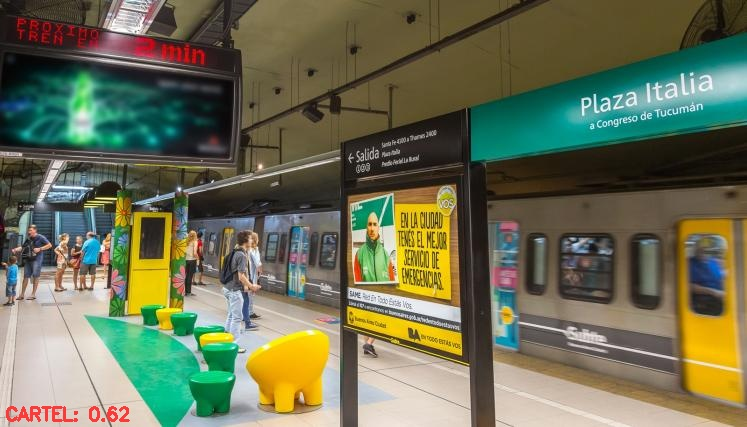
\includegraphics[width=0.6\textwidth]{./img/classif.jpg} }}
    \qquad
    \subfloat[\centering La detección de objetos indica \textit{dónde} está presente el objeto]{{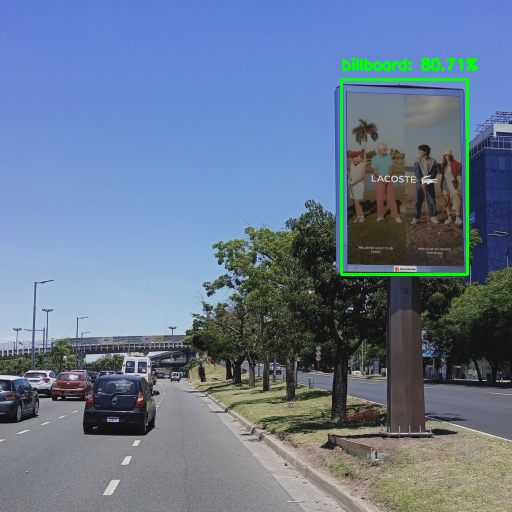
\includegraphics[width=0.6\textwidth]{./img/detection.jpg} }}
}
\end{figure}

El desafío principal de la detección de objetos es lograr una detección precisa, adaptada a todo tipo de imagen de entrada y que no se vea sesgada por el conocimiento previo tenido.

\subsection{Despliegue}

Originalmente nuestra propuesta mínima de trabajo fue desarrollar una herramienta de procesamiento de video pregrabado que se ejecute localmente por línea de comando y devuelva un video procesado como salida.

Si bien este era nuestro objetivo mínimo, consideramos que una de las principales metas del trabajo es entregar una experiencia de usuario con una interfaz mejor a la de línea de comando que pueda ser utilizado desde cualquier parte, sin requerir ningún tipo de instalación previa y que permitiera mostrar el video procesado en tiempo real.

La interfaz ideal que cumple con todos estos requisitos, es la de un sitio web.

El hecho de usar un sitio web para disponibilizar nuestro sistema nos da dos posibles arquitecturas a evaluar. Por un lado tenemos la arquitectura cliente-servidor, mientras que su contraposición natural es un sistema que sea ejecutado solamente en el cliente local.

En una arquitectura cliente-servidor, la capacidad computacional del cliente no es relevante, pero la complejidad principal del sistema recae en poder minimizar la latencia entre el cliente y el servidor.

Por otro lado, en una arquitectura sin servidor donde todo se ejecuta localmente, el principal desafío es poder seguir ofreciendo una buena experiencia de usuario independientemente del poder computacional del dispositivo sobre el cual corre el sistema.

\section{Resultado}

\subsection{\textit{BART}}

El resultado final del trabajo es \textit{\textbf{BART}} (Blocking Ads In Real Time), un \textit{software} accesible a través de una página web desplegada en \url{https://bart.fly.dev/}, el cual fue desarrollado en \url{https://github.com/bart-ai/bart/}.

El objetivo de esta página es tomar los cuadros de la cámara del dispositivo del usuario y poder procesarlos con nuestro sistema. El procesamiento de estos cuadros consiste en detectar si hay un anuncio presente (específicamente: un cartel publicitario), indicar en qué región del cuadro está presente el anuncio y presentarle esta detección al usuario.

\begin{figure}[H]
\makebox[\textwidth][c]{
    \subfloat{{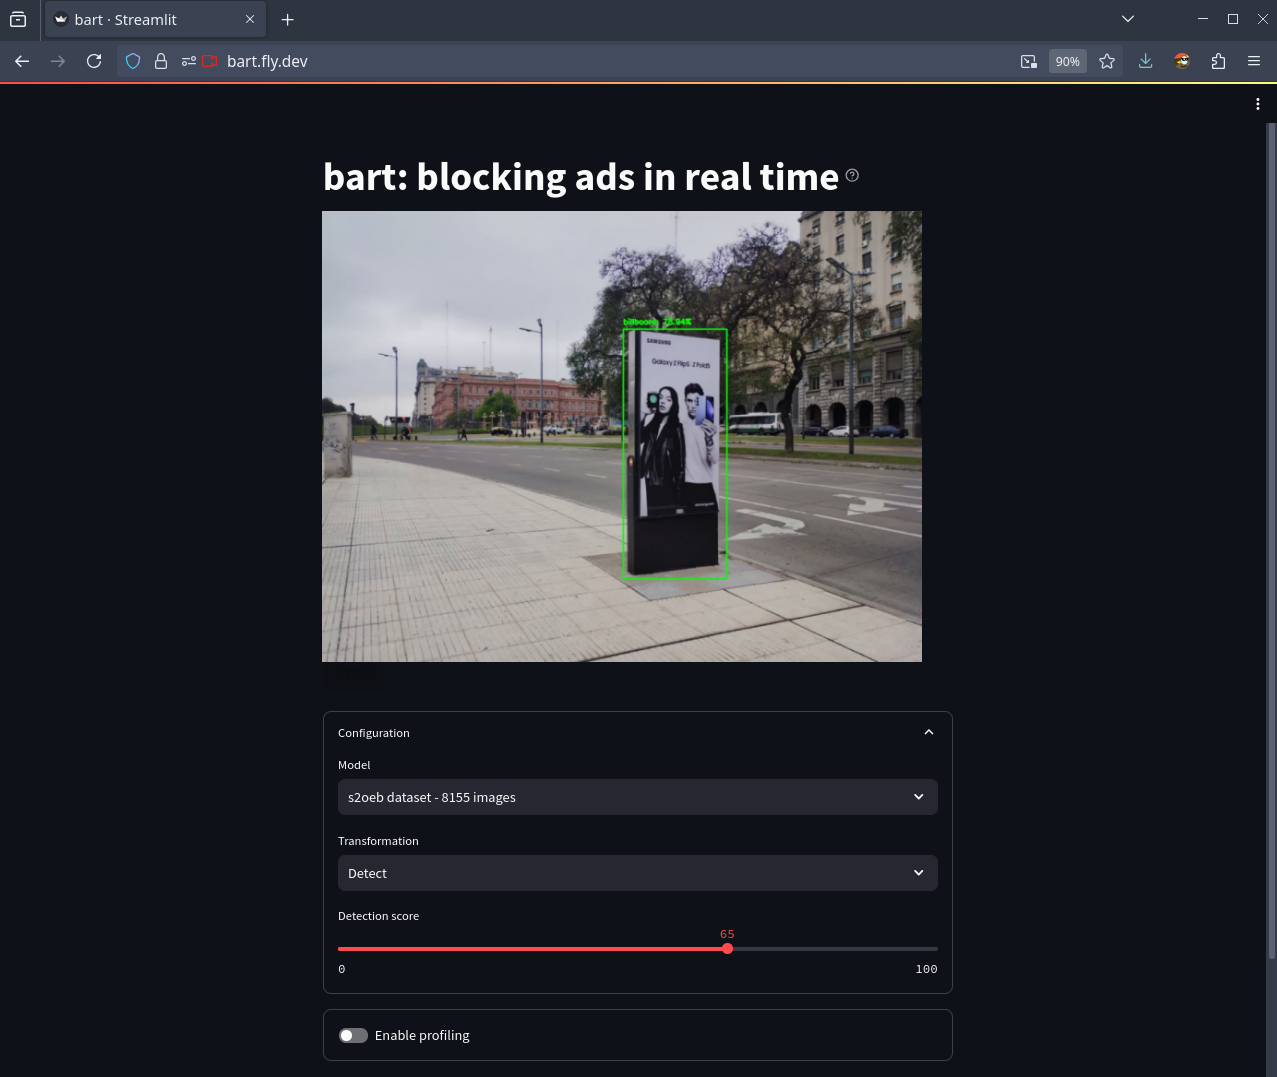
\includegraphics[width=0.7\textwidth]{./img/desktop.png} }}
    \qquad
    \subfloat{{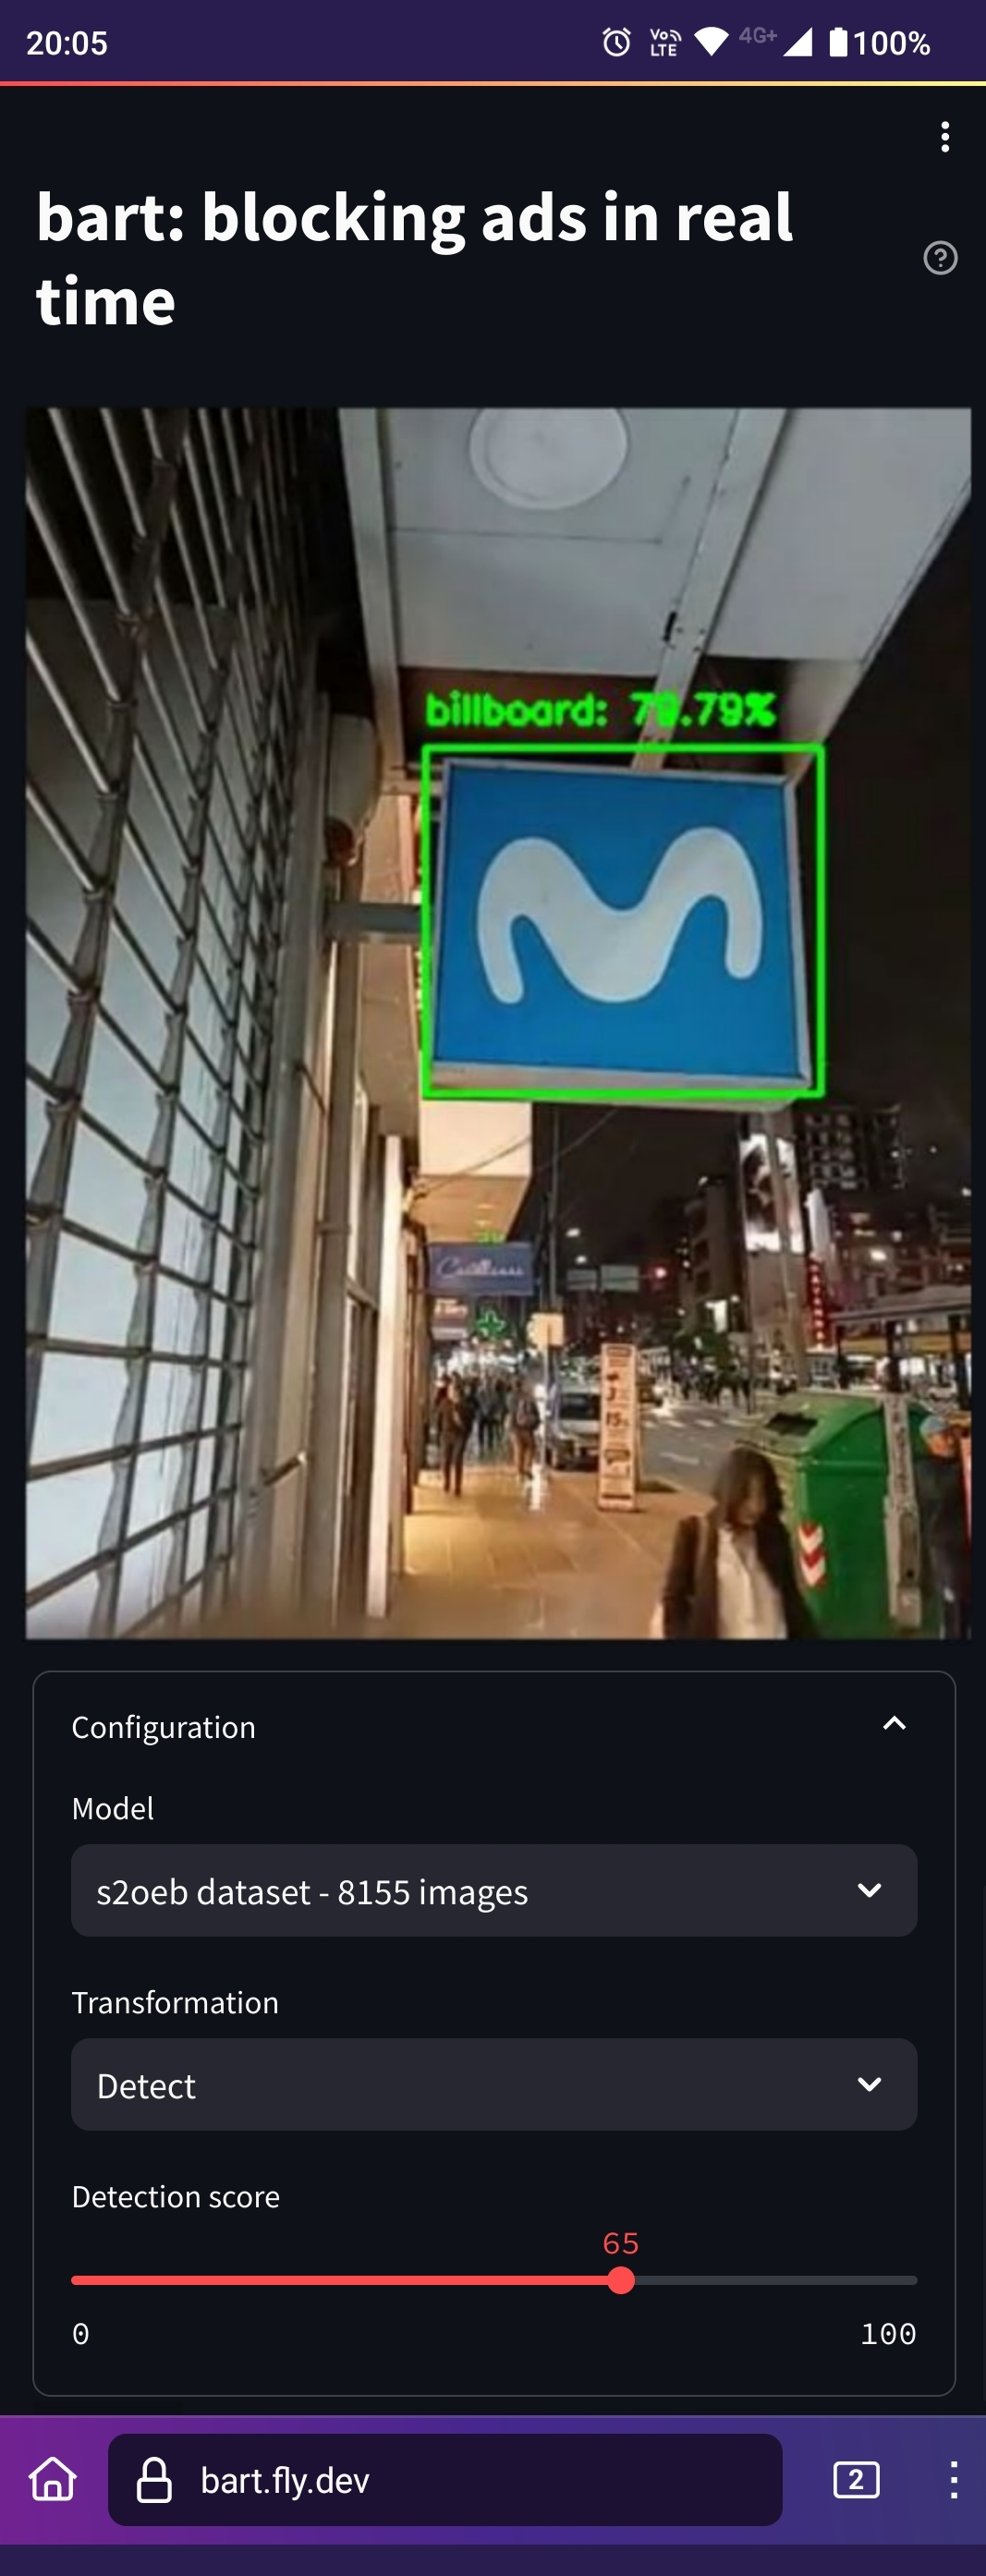
\includegraphics[width=0.22\textwidth]{./img/mobile.jpg} }}
}
\caption{Distintas disposiciones de \textit{BART} según las dimensiones del dispositivo}
\end{figure}

El contenido principal de la página es la sección donde se le muestra al usuario el video que está grabando con la cámara, con los anuncios detectados. Siendo la detección en la vía pública el principal caso de uso pensado para la aplicación, el sitio funciona correctamente en dispositivos portátiles y móviles, adaptándose a pantallas pequeñas, pero también provee un diseño para dispositivos con pantallas medianas o grandes lo cual es de gran utilidad para la prueba y el análisis de la eficiencia del sistema.

\subsubsection{Configuración del Sistema}

La página cuenta con una sección de configuración, donde el usuario puede elegir qué tipo de transformación se le aplica a los cuadros del video. Las transformaciones que provee el sitio son tres: solamente detectar objetos, difuminarlos, o incluso removerlos de la imagen. La naturaleza modular del sistema permite que sea sencillo agregar una transformación de imágenes en el futuro.

\begin{figure}[H]
\makebox[\textwidth][c]{
    \subfloat[\centering Detección]{{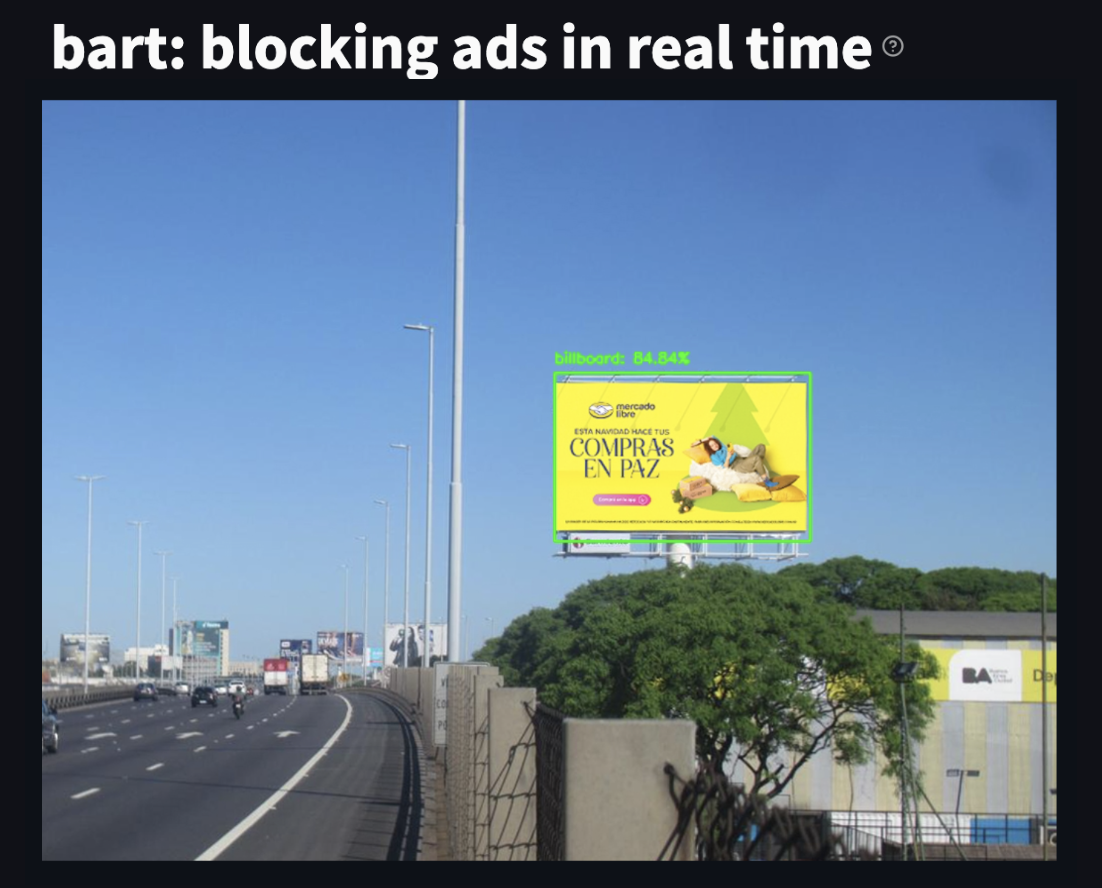
\includegraphics[width=0.4\textwidth]{./img/detect.png} }}
    \qquad
    \subfloat[\centering Difuminado]{{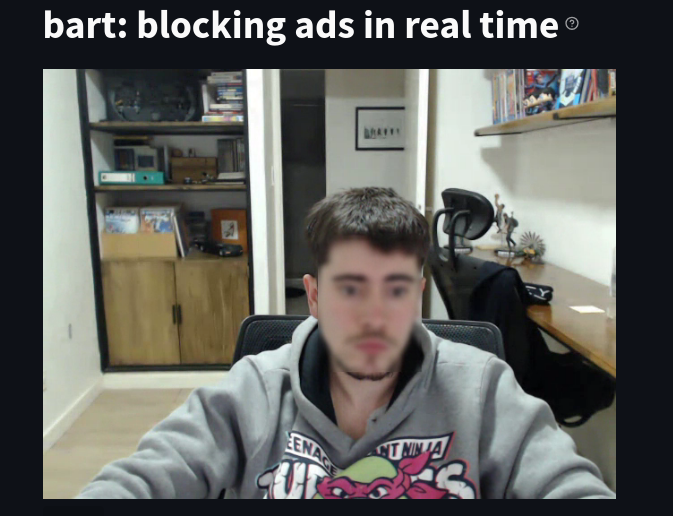
\includegraphics[width=0.4\textwidth]{./img/blur.png} }}
    \qquad
    \subfloat[\centering Eliminación]{{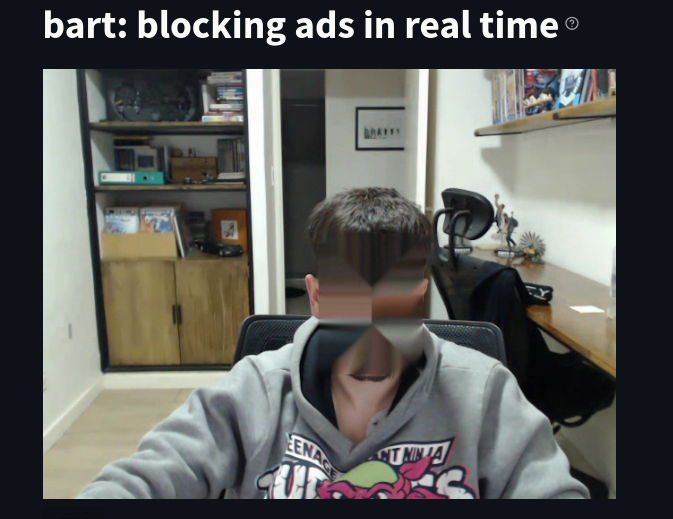
\includegraphics[width=0.4\textwidth]{./img/inpaint.png} }}
}
\end{figure}

Además, se le permite al usuario seleccionar el modelo a utilizar para la inferencia de objetos dentro de la imagen. Esto nos provee la posibilidad de comparar los distintos modelos sin tener múltiples despliegues, tener una manera sencilla de ver en tiempo real la efectividad de estos modelos, e incluso en un futuro poder probar modelos que detecten otro tipo de objetos que no sean carteles publicitarios (el sitio provee un detector facial a modo de ejemplo de esta modularización).

Finalmente, se puede configurar la confianza del modelo, lo cual le permite al usuario ser tan permisivo como le guste con las posibles detecciones del sistema.

\begin{figure}[H]
\makebox[\textwidth][c]{
    \subfloat[\centering Un valor alto de confianza es más estricto con las detecciones]{{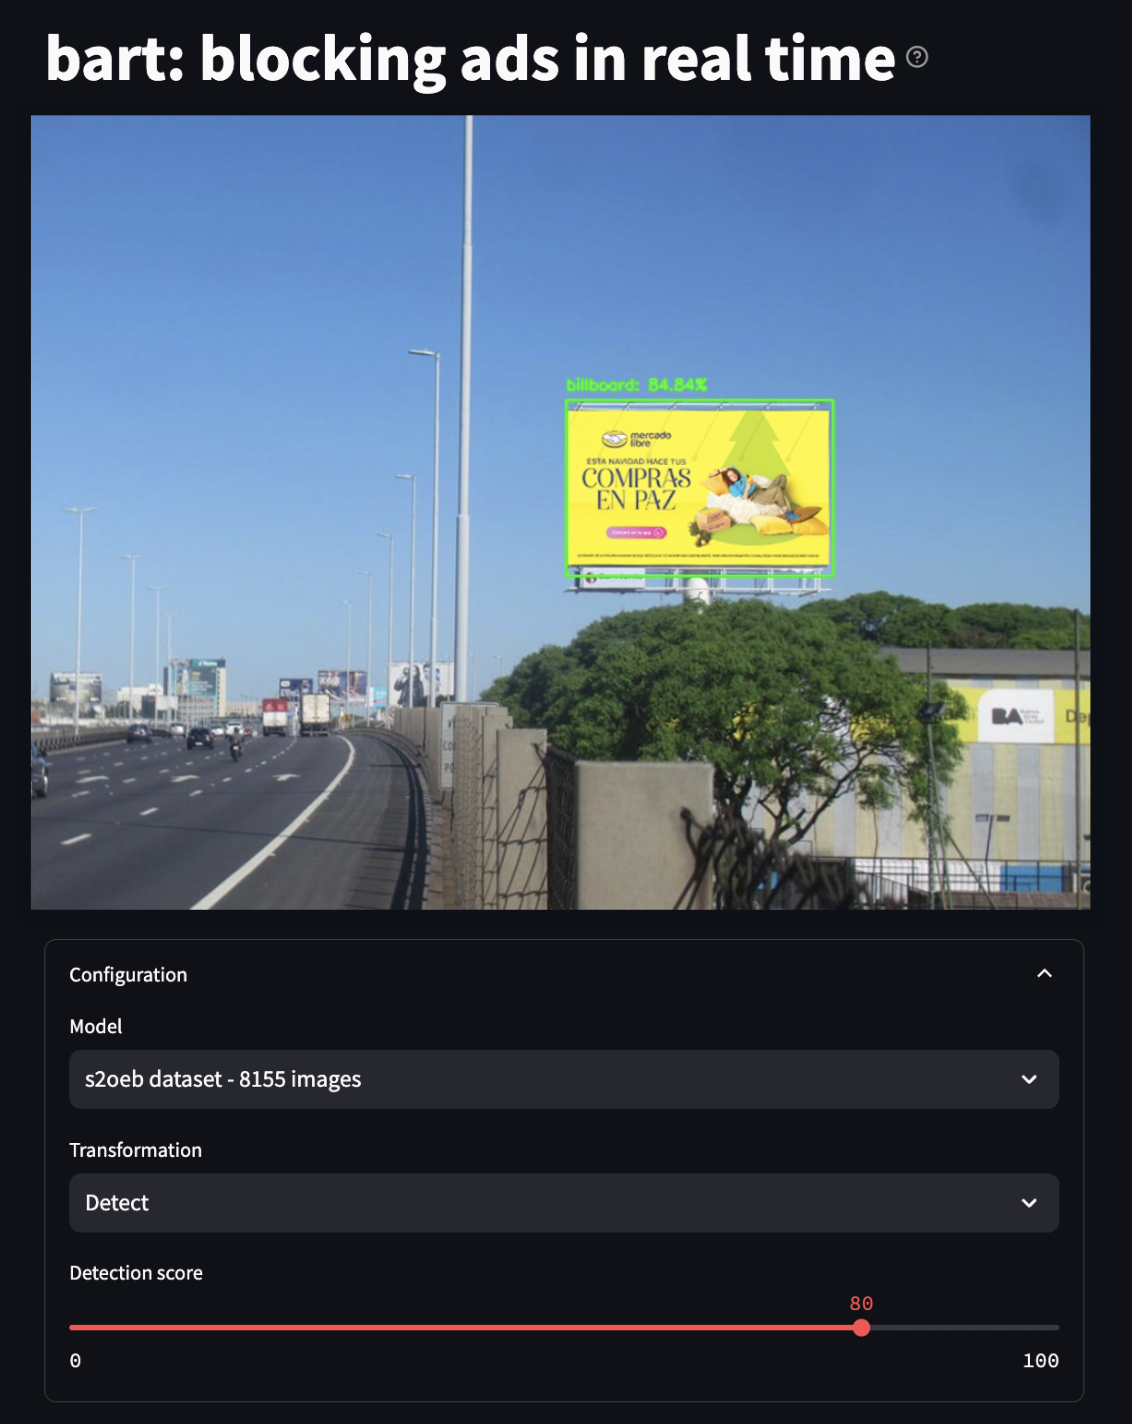
\includegraphics[width=0.45\textwidth]{./img/high-confidence.png} }}
    \qquad
    \subfloat[\centering Un valor bajo de confianza es más permisivo con las detecciones]{{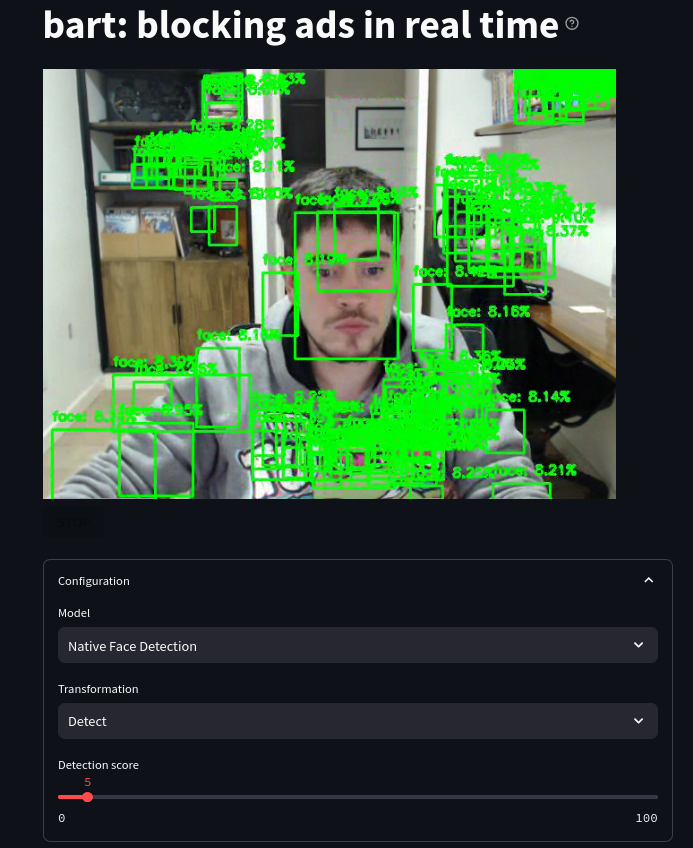
\includegraphics[width=0.45\textwidth]{./img/low-confidence.png} }}
}
\end{figure}

Todos los ajustes de configuración se hacen en vivo sobre el mismo sitio, es decir, no hace falta recargar ni la cámara del usuario ni el sitio en su totalidad, permitiendo una flexibilidad de qué y de cómo se detecta cada objeto, a medida que el sitio está en funcionamiento.

\subsubsection{Estadísticas}

El sitio además cuenta con una sección de estadísticas la cual sirve para poder comparar los modelos cualitativamente y no solamente quedarse con la sensación de cuán bien o mal está funcionando cada uno.

\begin{figure}[H]
\makebox[\textwidth][c]{
    \subfloat[\centering Medición de la velocidad de procesamiento del modelo con el tiempo]{{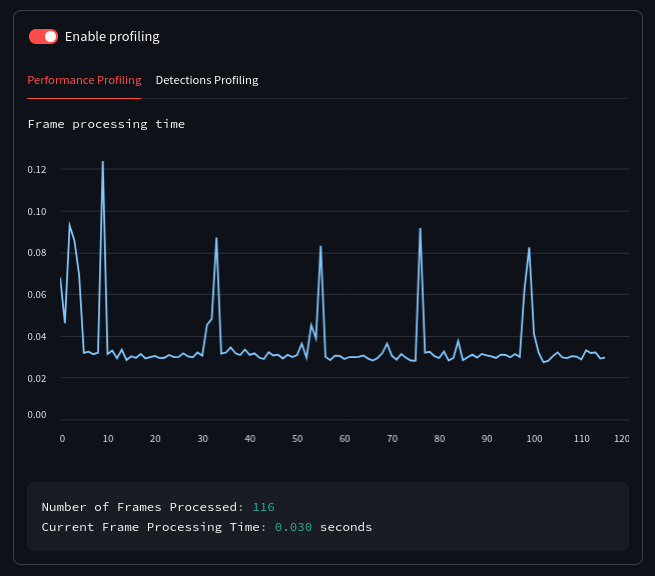
\includegraphics[width=0.5\textwidth]{./img/stats-perf.png} }}
    \qquad
    \subfloat[\centering Medición de las áreas de los objetos detectados con el tiempo]{{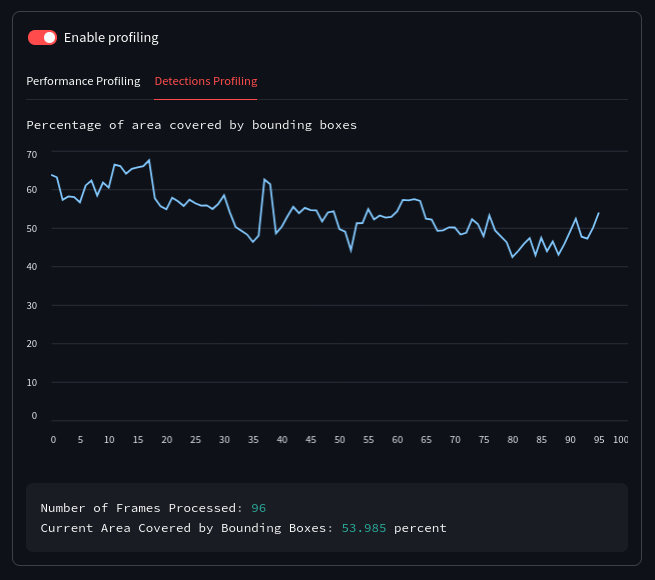
\includegraphics[width=0.5\textwidth]{./img/stats-area.png} }}
}
\end{figure}

Esta sección nos permite evaluar dos métricas importantes del modelo: la velocidad de detección sobre cada cuadro (y así saber qué modelo es más rápido que otro), y el tamaño del área detectada del objeto.

Esta última funcionalidad la ideamos con el fin de entender cuán presente está el objeto en cámara a medida que es filmado. Una pregunta interesante para hacerse, dado un anuncio, es si este está siendo muy disruptivo en lo que estamos queriendo ver o fotografiar. Esta funcionalidad nos permite obtener el área total del video que fue ocupada por el anuncio en cuestión.

\subsection{Detección de Anuncios}

\subsubsection{Redes Neuronales Conolucionales}

En \textit{Computer Vision}, la clasificación y detección de objetos en una imagen se hace a través de redes neuronales convolucionales.

Una red neuronal es un sistema de capas sucesivas donde cada capa procesa datos de entrada y el resultado es utilizado en la siguiente capa de la cadena hasta obtener el resultado final.

\begin{figure}[H]
\makebox[\textwidth][c]{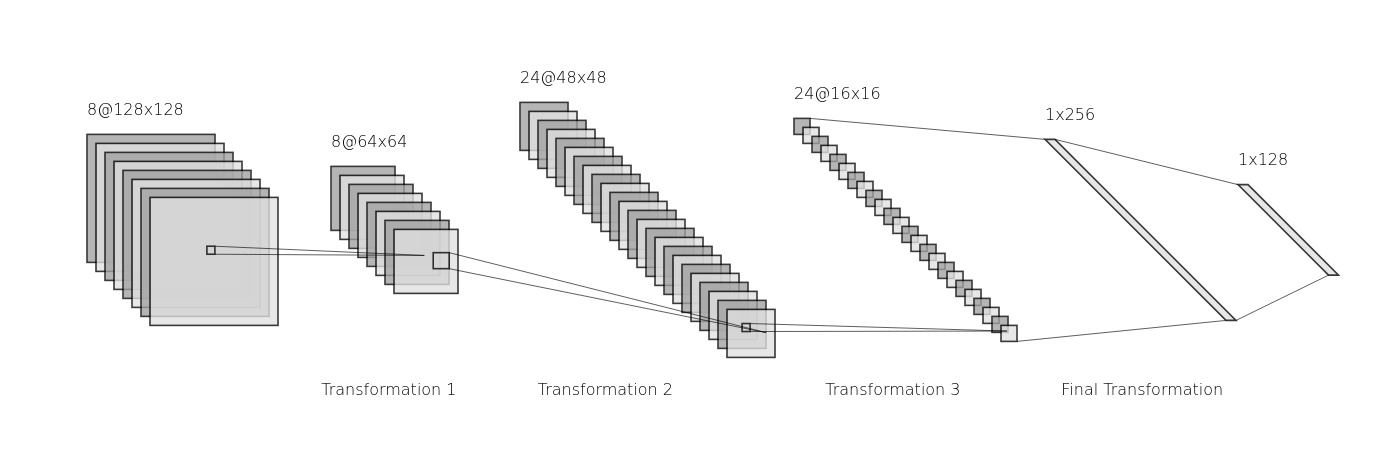
\includegraphics[width=1.2\textwidth]{./img/CNN.png}}
\caption{Ejemplo de una red neuronal de cinco capas}
\end{figure}


En el caso de las redes convolucionales los datos no son texto, sino que son imágenes.
Una imagen se codifica en forma de matriz: cada elemento representa un píxel y a su vez cada píxel es una representación numérica de sus colores.

\begin{figure}[H]
\makebox[\textwidth][c]{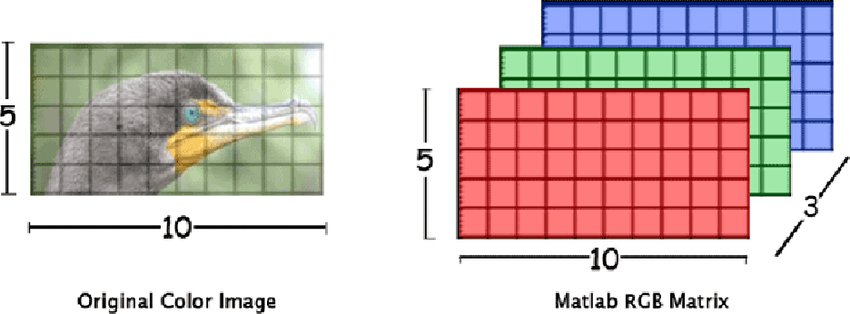
\includegraphics[width=0.7\textwidth]{./img/matrix.png}}
\caption{Una posible representación de una imagen es una matriz por cada canal de color (rojo, verde, azul)}
\end{figure}

Al ser los datos de entrada una matriz numérica, cada capa de la red neuronal debe realizar transformaciones mediante operaciones matriciales. La operación matemática fundamental de estas redes es la convolución: consiste en deslizar una matriz pequeña de filtro sobre la entrada y acumular los productos resultantes para producir una nueva matriz de salida, la cual se utilizará como entrada en la siguiente capa de la red.

\begin{figure}[H]
\makebox[\textwidth][c]{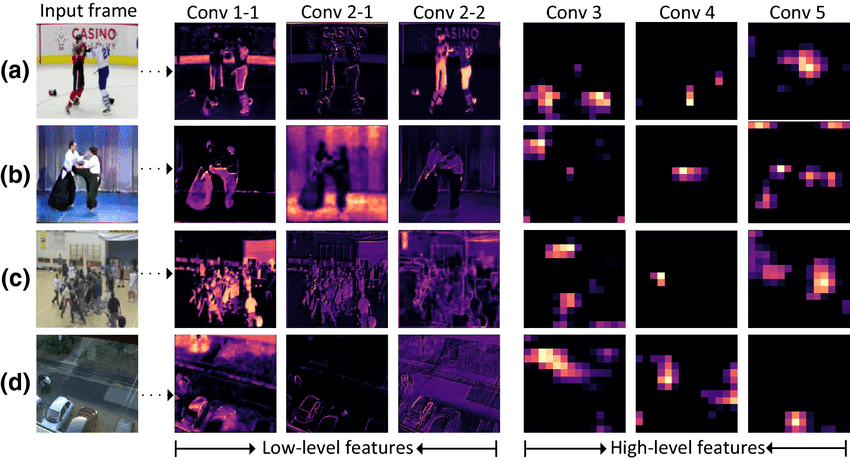
\includegraphics[width=0.9\textwidth]{./img/convolution.png}}
\caption{Las distintas convoluciones de cada capa nos permiten extraer características de la imagen}
\end{figure}

De esta manera, cada capa reduce la matriz original y extrae características relevantes de la imagen, permitiendo la detección de patrones en ella. Este proceso continua hasta tener un resultado final de las características aprendidas.

\begin{figure}[H]
\makebox[\textwidth][c]{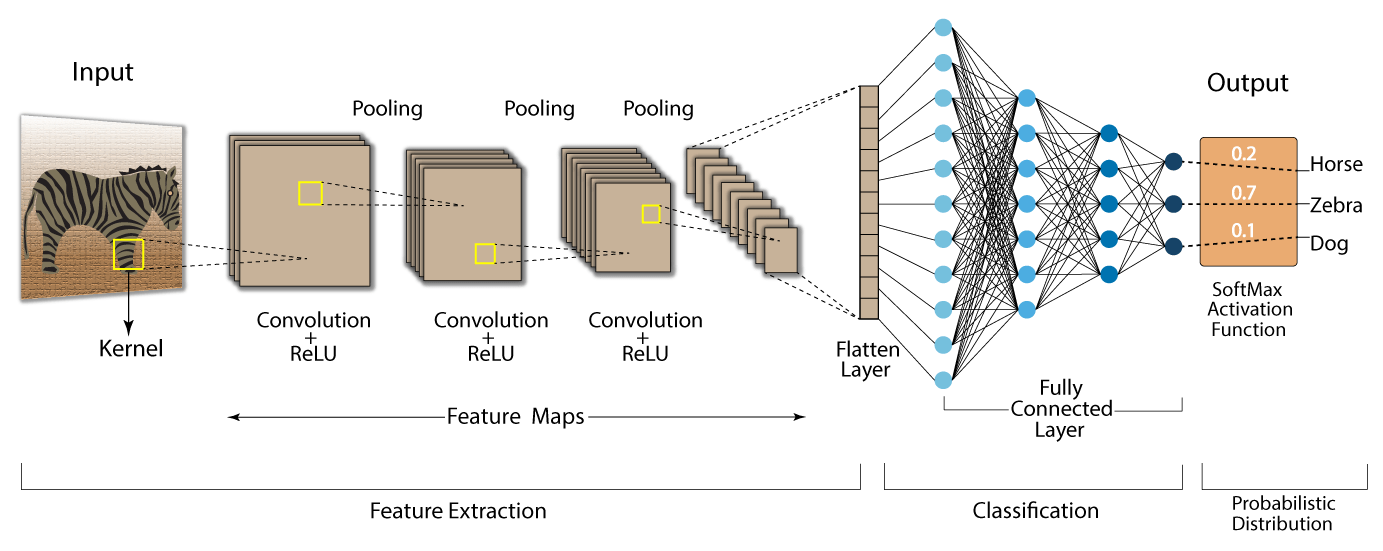
\includegraphics[width=\textwidth]{./img/cnn-skel.png}}
\caption{Una \textit{CNN} toma una imagen de entrada y luego de varios pasos termina en una clasificación de esta}
\end{figure}

\subsubsection{\textit{Transfer Learning}}

En los últimos años, el campo de la inteligencia artificial avanzó en niveles exponenciales, no solo con conceptos y tecnologías nuevas, sino que además mejorando considerablemente la experiencia de usuario, permitiéndole a los desarrolladores de \textit{software} no necesitar ser expertos en la disciplina para poder experimentar con los últimos avances.

Si bien es posible desarrollar a bajo nivel, donde se puede diseñar la arquitectura de una red neuronal y luego entrenar un modelo partiendo desde cero, lo más usual es la refinación sobre modelos ya existentes. \textit{Transfer Learning} es exactamente eso: partir de un modelo existente y adecuarlo a un nuevo problema. Tomando un modelo generalista de detección de objetos, se utilizan datos de clases de objetos específicos para entrenar un nuevo modelo que cumpla las necesidades del proyecto.\\

Partiendo desde un modelo pre-entrenado basado en la familia de algoritmos \textit{YOLO}, nuestro trabajo consiste en optimizar el entrenamiento de un nuevo modelo que cumpla nuestros requerimientos específicos: en nuestro caso, detección de carteles publicitarios.

\textit{YOLO}, \textit{You Only Look Once} \cite{yolov1}, es un tipo de algoritmo de detección de objetos en tiempo real introducido en 2016 que rápidamente demostró ser una alternativa superior a los métodos existentes. A diferencia de otros métodos de detección de objetos que pasan una imagen a través de la red varias veces, \textit{YOLO} realiza todas las predicciones con una sola pasada a través de la red, lo que lo hace extremadamente rápido y la mejor opción para nuestro trabajo.

En nuestro caso hicimos uso de la implementación de \textit{YOLO} que ofrece \textit{Ultralytics} \cite{ultralytics}, denominada \textit{YOLOv8}. Además del algoritmo, \textit{Ultralytics} provee un entorno de \textit{software} que permite refinar modelos pre-entrenados, evaluarlos, y compararlos.

\subsubsection{Entrenamiento de la Red}

El entrenamiento de una red convolucional partiendo de un modelo pre-entrenado consiste en utilizar un \textit{dataset} de imágenes nuevo que se ajuste a las especificidades del nuevo problema. En nuestro caso necesitamos obtener distintos \textit{dataset} de imágenes de entrenamiento que contenga carteles publicitarios en la vía pública.

Considerando que queremos partir de una cantidad considerable de imágenes para el entrenamiento, si bien una de las posibilidades que se presentan en este tipo de proyectos es tomar las fotos de manera manual, lo más usual es recurrir a conjuntos de datos ya curados para otros proyectos que se adecuen a nuestros propósitos. Un portal que deja a disposición distintos \textit{datasets} públicos es \textit{Roboflow} \cite{roboflow} y de allí tomamos las imágenes deseadas.\\

Como punto de comparación y caso de estudio para comprender el proceso, se tiene un modelo pre-entrenado sobre el \textit{dataset} \textit{Open Images} \cite{openimages}, un conjunto de datos clasificado en múltiples tipos de objetos (autos, animales, carteles, etc.), el cual fue de gran uso al comenzar el proyecto cuando no se disponía de un modelo propio.

\subsubsection{Interpretación del Modelo}

La interpretación de un modelo es un proceso enteramente separado de su construcción que consiste en la \textbf{inferencia}: ejecutar el modelo sobre información nueva y tomar conclusiones de esta.

Independientemente del armado del modelo, se debe tener un sistema en funcionamiento para su lectura y ejecución sobre las imágenes a predecir, que no necesariamente debe utilizar las mismas herramientas que se usaron en el entrenamiento de este.

Para las tareas de manipulación de imágenes y la inferencia sobre ellas la principal herramienta que utilizamos es \textit{OpenCV} \cite{opencv}: una biblioteca de funciones especializada en \textit{Computer Vision} que provee un entorno de desarrollo en \textit{Python}, el lenguaje de programación utilizado en todo el proyecto.

\subsection{Despliegue Web}

Como mencionamos previamente, el objetivo del trabajo es disponibilizar la aplicación a través de una página web. Esto nos llevó a considerar dos alternativas de arquitectura, una donde el cliente envía el video y la detección ocurre en un servidor centralizado, y la otra donde la detección se produce en el dispositivo local sin salir del cliente en ningún momento. Parte del trabajo fue la evaluación de ambas arquitecturas y decidir cuál es la que mejor se adapta a nuestras necesidades.

\subsubsection{Detección en el Cliente}

Inicialmente creíamos que la velocidad de la red nunca iba a ser suficiente para soportar una arquitectura cliente-servidor, por lo tanto comenzamos probando hacer la detección exclusivamente en el cliente.

Buscando interoperabilidad entre el entorno web y los lenguajes de programación de desarrollo que no afectara el rendimiento resultante, recurrimos a \textit{WebAssembly} \cite{wasm}. \textit{WASM} es un estándar en crecimiento de adopción desarrollado para ejecutarse dentro de navegadores web, sin importar el lenguaje de desarrollo, ya que implica una compilación del lenguaje de entrada a instrucciones binarias.\\

Utilizando \textit{Pyodide} \cite{pyodide}, un compilador de \textit{Python} a \textit{WebAssembly}, se pudo obtener una prueba de concepto del sitio web que se ejecutara enteramente en el dispositivo, sin depender de un servicio externo. Lamentablemente, la compilación de \textit{Python} a \textit{WASM} implica compilar el intérprete completo de \textit{Python} en vez de solamente las instrucciones de nuestro sistema. Esto provoca un rendimiento extremadamente por debajo de lo deseado, lo cual muestra una de las grandes falencias de \textit{WebAssembly}: si bien el objetivo final del estándar es ejecutar cualquier lenguaje de programación en un explorador web, el rendimiento es aceptable solamente en lenguajes compilados (\textit{Rust}, \textit{Go}, \textit{C}) y no interpretados (\textit{Python}), al menos hasta que se encuentre una solución que no involucre compilar intérpretes completos.

\subsubsection{Detección en el Servidor}

Habiendo descartado la alternativa de hacer la detección en el cliente, solamente nos quedaba la opción de utilizar un servidor centralizado para hacer las detecciones.

Frente a una arquitectura cliente-servidor es fundamental la velocidad de conexión con la que el cliente se conecta con el servidor, y mitigar que una conexión lenta produzca una demora considerable en la comunicación entre ambos componentes.

Necesitamos mandar los cuadros al servidor para que este pueda detectarlos y luego mandarlos al cliente de vuelta, quien recién ahí puede mostrarlos al usuario. Es importante que esto suceda rápido dado que de lo contrario se perdería el componente de ``tiempo real'' y el video resultado aparecería muy desfasado de la realidad.

Este requerimiento colisiona directamente con nuestra idea de que la aplicación será usada principalmente en la vía pública, dado que es el lugar donde peor conexión uno va a tener comparado a una conexión \textit{WiFi} estable en un hogar.\\

Para lograr una detección en tiempo real hicimos uso de \textit{WebRTC} \cite{webrtc}. Se trata de un protocolo moderno que permite comunicaciones par-a-par y en tiempo real, con interfaces nativas del navegador, por lo que no requiere ningún tipo de complemento. Es utilizado principalmente en aplicaciones de llamadas de voz, video, chat y para compartir archivos entre navegadores.

Utilizando \textit{WebRTC} como el motor de streaming de video pudimos lograr una comunicación rápida y eficiente en recursos entre el navegador cliente de la aplicación y nuestro servidor centralizado que hace las detecciones.

\subsubsection{\textit{Hosting} en la Nube}

En consecuencia de optar por una arquitectura cliente-servidor, se necesita tener al sistema disponible, alojado en un servidor accesible desde cualquier lado.

Para poner en funcionamiento nuestro sistema utilizamos \textit{Fly.io} \cite{flyio}, una plataforma como servicio (\textit{PaaS}) que nos permite desplegar el código en servidores distribuidos geográficamente en varios lugares, lo que nos permitió poder alojar físicamente nuestro servidor cerca de los usuarios de la aplicación, y así reducir la latencia de comunicación entre el dispositivo y el servidor.

\section{Implementación}

La implementación del sistema final tiene tres componentes principales. Por empezar, se tuvo que desarrollar un flujo que nos permitiera experimentar en el armado de modelos de redes neuronales convolucionales, comenzando por definir de qué manera podemos decidir que un modelo es apto para el sistema y utilizando herramientas para la comparación entre los distintos experimentos. Por otro lado tenemos la lectura que se hace de estos modelos, utilizándolos para inferir sobre videos del usuario. Para finalizar, integrando ambas partes y proveyendo una presentación del sistema en su totalidad, se evaluaron distintas alternativas del despliegue web que une todas las partes.

\subsection{Modelo}

\subsubsection{¿Qué es un buen modelo?}

Para lograr un sistema de detección que satisfaga las demandas del proyecto, fue necesario definir qué atributos de calidad deben ser priorizados y utilizados para la comparación de las distintas alternativas e ideas que vayan surgiendo.\\

Los atributos de calidad priorizados para nuestros modelos son:

\begin{itemize}
\itemsep0em
    \item Velocidad de procesamiento
    \item Precisión de la inferencia
\end{itemize}

Un modelo óptimo para nuestro caso de uso debe balancear correctamente estos dos atributos, ya que un sistema que se demore significativamente en procesar cada cuadro, por más preciso que sea, no cumpliría nuestra meta de ser en tiempo real; mientras que un sistema que no logre detecciones acertadas, por más rápido que sea, no cumpliría el objetivo central de la inferencia.

Como veremos en múltiples partes del sistema (tanto de la parte del modelo como del resto), la velocidad y la precisión son dos atributos que están interrelacionados entre sí y se presentan constantemente como una contrapartida del otro. Técnicas que ayuden a mejorar uno de los dos atributos frecuentemente disminuyen la calidad del otro, y viceversa.

\subsubsection{Velocidad del procesamiento}

La velocidad de un modelo se puede medir por la cantidad de segundos que se toma en procesar una imagen.

Al ser este modelo parte de un sistema de procesamiento de videos, no debemos pensar en imágenes individuales, sino que debemos considerar cada entrada como una parte del todo: un fotograma de un video. Por lo tanto, la métrica relevante para saber cuán viable es un modelo dentro de nuestro proyecto es el agregado de cuánto se demora en procesar el conjunto de cuadros recibidos.

\subsubsection{Precisión de la Inferencia}

La precisión del modelo debe englobar distintos tipos de aciertos y errores. Lo que se debe contabilizar es la combinación entre las predicciones hechas y su correctitud. Es decir, nos importa medir tanto cuán correctas fueron las predicciones hechas, pero también qué predicciones se debieron hacer pero no se hicieron. Este concepto se conoce como la confusión del modelo y se puede visualizar en una grilla que combine estos dos atributos.

\begin{figure}[H]
\makebox[\textwidth][c]{
    \captionsetup{margin=0cm}
    \subfloat[\centering Un \textit{falso negativo} es un \textbf{error} donde no se detectó un objeto que sí esta presente]{{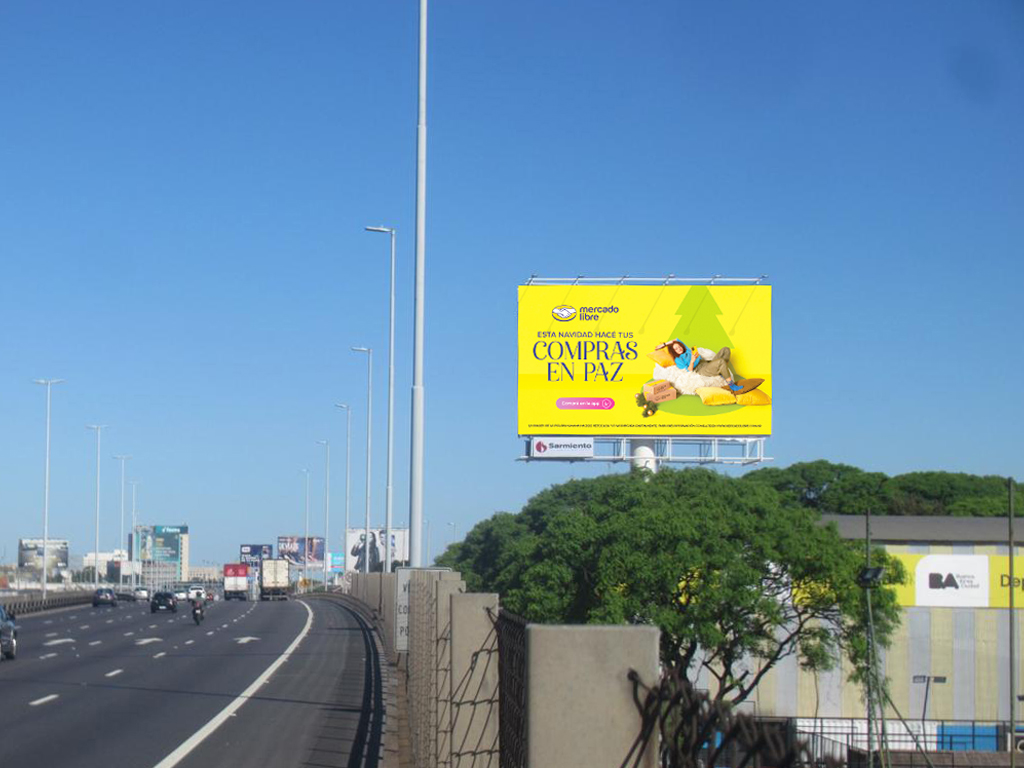
\includegraphics[width=0.5\textwidth]{./img/FN.jpg} }}
    \qquad
    \subfloat[\centering Un \textit{verdadero negativo} es un \textbf{acierto} donde no se detecta ningún objeto ya que realmente no hay ninguno presente]{{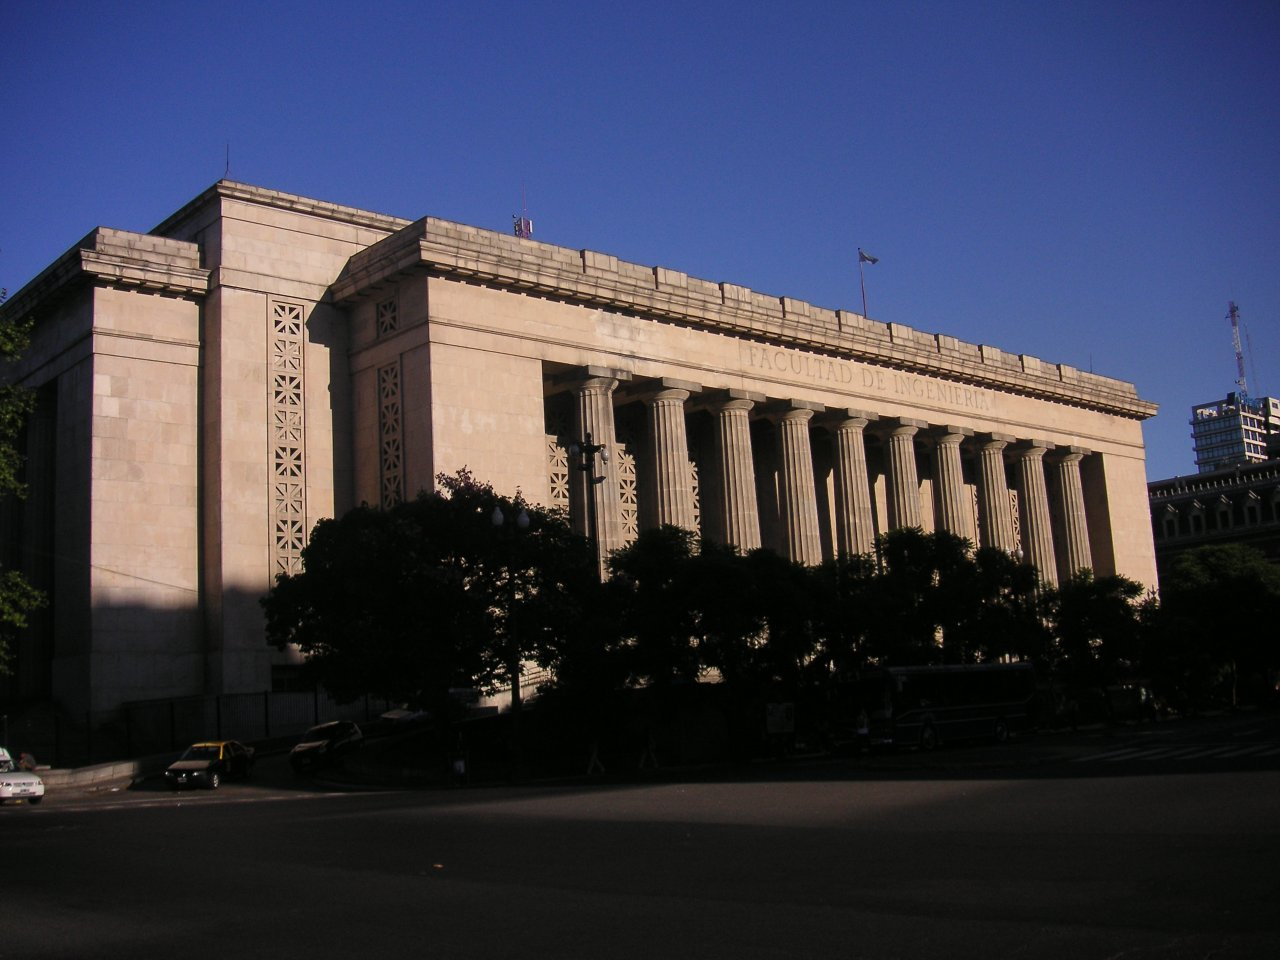
\includegraphics[width=0.5\textwidth]{./img/TN.jpg} }}
}
\end{figure}

\hrule

\begin{figure}[H]
\makebox[\textwidth][c]{
    \captionsetup{margin=0cm}
    \subfloat[\centering Un \textit{verdadero positivo} es el \textbf{acierto} donde se detecta un objeto correctamente]{{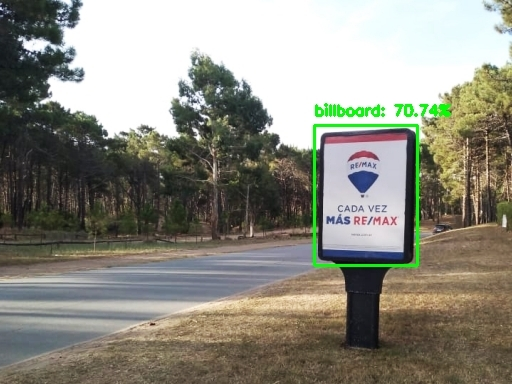
\includegraphics[width=0.5\textwidth]{./img/TP.jpg} }}
    \qquad
    \subfloat[\centering Un \textit{falso positivo} es un \textbf{error} donde se detecta un objeto no presente en la realidad]{{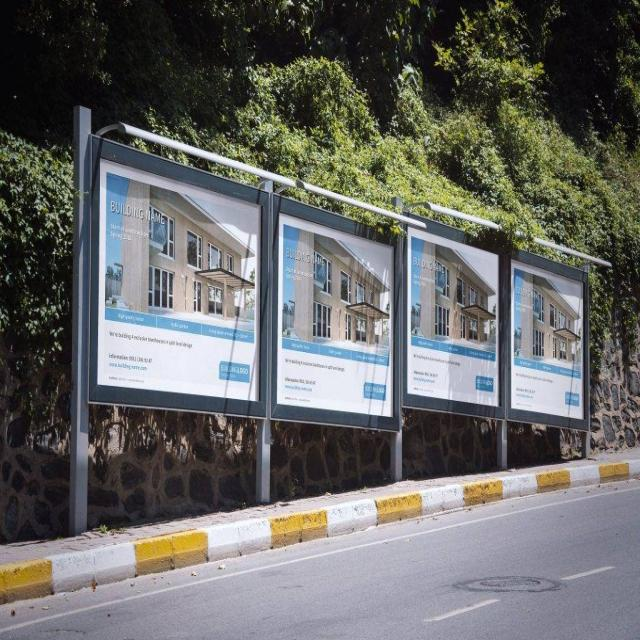
\includegraphics[width=0.5\textwidth]{./img/FP.jpg} }}
}
\end{figure}

Entender si una predicción es correcta o no, dentro del área de detección de objetos en imágenes, no es una tarea simple. Un modelo que detecta objetos dentro de imágenes va a dar como resultado el mínimo rectángulo que contiene al objeto deseado, y este resultado debe ser comparado contra el rectángulo verdadero donde se ubica el objeto.\\

La comparación entre estos dos rectángulos (la predicción, y la realidad) nos provee dos piezas de información que determinan cuán correcta es la predicción:

\begin{itemize}
\itemsep0em
    \item La superposición de ambos rectángulos, es decir su \textbf{intersección}, nos revela qué tan bien el rectángulo predicho coincide con el rectángulo verdadero. Una mayor intersección indica una mayor precisión en la localización del objeto.
    \item La suma total de las áreas de ambos rectángulos, es decir la \textbf{unión}, nos muestra el área combinada que ocupan los rectángulos de lo predicho y lo verdadero. Esto nos ayuda a entender el grado de error de la predicción, considerando tanto las áreas correctamente identificadas como las áreas incorrectamente tenidas en cuenta.
\end{itemize}

La combinación de estas métricas se conoce como la Intersección sobre la Unión (\textit{IoU}, \textit{Intersection over Union}), y nos provee un único número que varía entre 0 y 1. Un valor de \textit{IoU} de 1 indica una predicción perfecta, mientras que un \textit{IoU} de 0 indica que no hay superposición entre los rectángulos.

\begin{figure}[H]
\makebox[\textwidth][c]{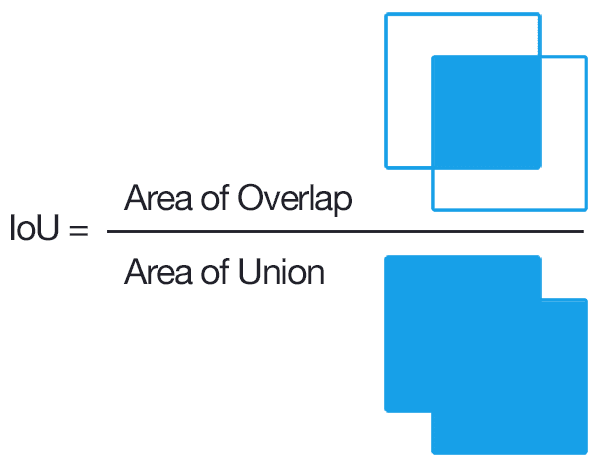
\includegraphics[width=0.4\textwidth]{./img/iou.png}}
\caption{Intersección sobre la Unión}
\end{figure}

Para medir la precisión, se necesita decidir un umbral a partir del cual será considerada como correcta. Por ejemplo, si queremos obtener la precisión promedio con \textit{IoU} 0.5, solo contaremos como correctas las predicciones para las cuales el \textit{IoU} es mayor a 0.5.

\begin{figure}[H]
\makebox[\textwidth][c]{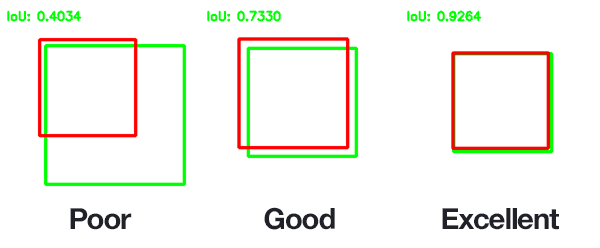
\includegraphics[width=0.6\textwidth]{./img/iou-examples.png}}
\caption{Ejemplos de distintos valores de \textit{IoU}}
\end{figure}

Dado que la calidad de una predicción es una escala, no nos sirve quedarnos solamente con la precisión con \textit{IoU} 0.5. Lo que se busca es medir la precisión del modelo en varios niveles de \textit{IoU} y luego promediarlos, para obtener una métrica que nos permite comparar dos modelos distintos. Esta métrica se denomina \textit{Mean Average Precision} (\textit{mAP}) y es utilizada frecuentemente en evaluación y comparación de modelos de redes neuronales ya que cumple el objetivo de proporcionar una evaluación amplia y completa del rendimiento del modelo.

Utilizando un umbral entre 0.5 y 0.95 para esta métrica (denominado \textit{mAP50-95}), obtenemos un valor numérico que nos indique qué tan efectivo es un modelo en comparación con otros y así poder evaluar y seleccionar el mejor modelo a utilizar en nuestro sistema.

\subsubsection{Base del Entrenamiento}

Como mencionamos previamente, la arquitectura de una red neuronal convolucional consiste de capas que aplican transformaciones hasta llegar a un resultado final. Mientras más capas tenga una red, mejor va a ser la precisión y calidad de la inferencia, ya que extrae más información de los datos de entrada. Naturalmente, debido al agregado al proceso, aumentar la cantidad de capas también va a hacer más lenta cada inferencia. Es decir, un sistema de inferencia con más capas tiende a ser más preciso, a costa de que sea un procesamiento más intensivo y por ende más lento.

Es por esto que es muy importante elegir correctamente la arquitectura de la red neuronal del modelo, teniendo en cuenta lo que el proyecto requiere, ya sea un sistema lento pero preciso, un sistema veloz pero de menor calidad de inferencia, o un balance que tenga en consideración ambos atributos. \\

La implementación \textit{YOLOv8} de \textit{Ultralytics} no solo permite entrenar un modelo de una red neuronal sin base alguna, sino que también ofrece distintos modelos basados en redes de distintos tamaños (\textit{nano}, \textit{small}, \textit{medium}, \textit{large} y \textit{xlarge}) donde cada modelo base se adapta a diferentes necesidades y recursos computacionales.

Durante el proceso de desarrollo exploramos entrenar modelos partiendo desde todas las categorías. Rápidamente notamos que nos iba a ser imposible ofrecer procesamiento en tiempo real con un modelo a base de los modelos \textit{large} o \textit{xlarge} dado que su velocidad de procesamiento de imagen era demasiado lenta para nuestros requerimientos. Si bien estas redes son de gran utilidad en entornos donde la precisión es la prioridad máxima, no son compatibles con nuestro caso de uso.

Finalmente, el modelo pre-entrenado que mejor se ajustó a nuestras necesidades es el de tamaño \textit{nano}. Partiendo de este modelo logramos una detección notablemente más veloz que con los tamaños \textit{small} y \textit{medium}, sin una pérdida de precisión relevante.

\subsubsection{Entrenamiento}

Además de la arquitectura de la red, un componente primordial en el modelo resultante es su entrenamiento. Es el proceso principal utilizado sobre el modelo para lograr inferencias precisas y de calidad.

Para los problemas de detección de objetos se utiliza un sistema de entrenamiento supervisado. Esto significa que por cada predicción que el modelo haga durante la etapa de entrenamiento uno ya conoce el resultado correcto y puede comparar la predicción del modelo contra lo que conoce, permitiéndole ajustar el modelo de acuerdo a si acertó o no.

El conjunto total de los datos que se usan para entrenar se debe dividir en tres subconjuntos: \textit{train}, \textit{test} y \textit{validate}.\\

La mayoría de los datos deberán ir en el subconjunto de \textit{train} ya que son las predicciones que el modelo hará en las iteraciones de entrenamiento. Es importante tener un conjunto de \textit{train} con un volumen grande de datos, con sus resultados bien clasificados y que sean imágenes de buena calidad, lo más similar posible a la realidad que queremos modelar.

El subconjunto de \textit{validate} se utiliza para evaluar al modelo luego de una cierta cantidad de iteraciones del entrenamiento y así poder recalibrarlo a medida que avanza el proceso. De esta forma se garantiza que el modelo no esté simplemente memorizando los datos de entrenamiento, sino que esté aprendiendo patrones que puedan generalizarse a nuevos datos.

Una vez finalizadas las iteraciones de entrenamiento se va a utilizar el subconjunto de \textit{test} para obtener la precisión del modelo en ejemplos que nunca vio. Es importante que usemos datos para \textit{test} que no se encuentran ni en \textit{validate} ni en \textit{train} dado que sino estaríamos probando el modelo contra resultados que ya conoce, en vez de evaluar su rendimiento en ``el mundo real''. Dado que nos es crucial comparar distintos modelos entre sí, es fundamental que en esta etapa utilicemos los mismos datos para todos los modelos entrenados en el sistema, en vez de utilizar distintos subconjuntos para cada modelo, ya que de esta manera podemos garantizar una evaluación consistente y objetiva de qué modelo funciona mejor.\\

Una etapa opcional aplicada en el proceso de entrenamiento del modelo es el ajuste de hiperparámetros (o \textit{Hyperparameter Tuning}), donde se busca determinar la configuración óptima para el entrenamiento del modelo sobre el dataset particular que se utilice. Este procedimiento es fundamental para maximizar el rendimiento del modelo, ya que distintas combinaciones de hiperparámetros pueden resultar en entrenamientos muy diversos. No existe una configuración perfecta que sea universalmente aplicable a todos los modelos sobre todos los \textit{datasets}, sino que es necesario explorar diversas combinaciones de valores y evaluar cuál se adapta mejor a las necesidades específicas del proyecto en cuestión.\\

El entrenamiento es un proceso muy costoso en el cual se invierten recursos computacionales y mucho tiempo, llegando a tomar múltiples días para poder finalizar un solo experimento. El aprendizaje supervisado no es un problema que se puede solucionar simplemente dedicando más horas al entrenamiento: un entrenamiento de 72 horas puede dar los mismos resultados que uno de 2 horas.

Más allá de los avances de \textit{hardware}, el ámbito de \textit{Machine Learning} está constantemente evolucionando para optimizar estos procesos. En particular existe el método \textit{Incremental Learning}, el cual consiste en mejorar iterativamente un modelo de aprendizaje supervisado entre sesiones de entrenamiento. En las redes neuronales convolucionales este método se aplica al utilizar las capas convolucionales de la red pero sin utilizar las capas finales de clasificación, así congelando al modelo parcialmente y pudiendo hacer que el entrenamiento posterior tome ventaja de la información ya aprendida. Sin embargo este proceso es muy complejo y da lugar a problemas como el \textit{Catastrophic Forgetting}, donde un modelo olvida lo aprendido previamente y solo tiene en cuenta los datos más recientes. Es por su complejidad que este método todavía no está enteramente desarrollado en el campo de \textit{Computer Vision} y no es parte del trabajo.

\subsubsection{Datos del Entrenamiento}

Una parte grande de nuestro trabajo consistió en construir un gran conjunto de datos de buena calidad y que se ajuste a la realidad que buscamos modelar: carteles publicitarios en la vía pública. Utilizando \textit{Roboflow}, obtuvimos varios conjuntos de datos de distintos tamaños y los combinamos de varias maneras para entrenar nuestros modelos. Esto no solo nos ayudó a construir un conjunto de datos suficientemente grande, sino que además nos permitió mitigar sesgos sobre los datos, evitando reducirnos a utilizar carteles de un único país, o sobre un contexto limitado (por ejemplo, solo utilizar carteles de autopistas)

\begin{figure}[H]
\makebox[\textwidth][c]{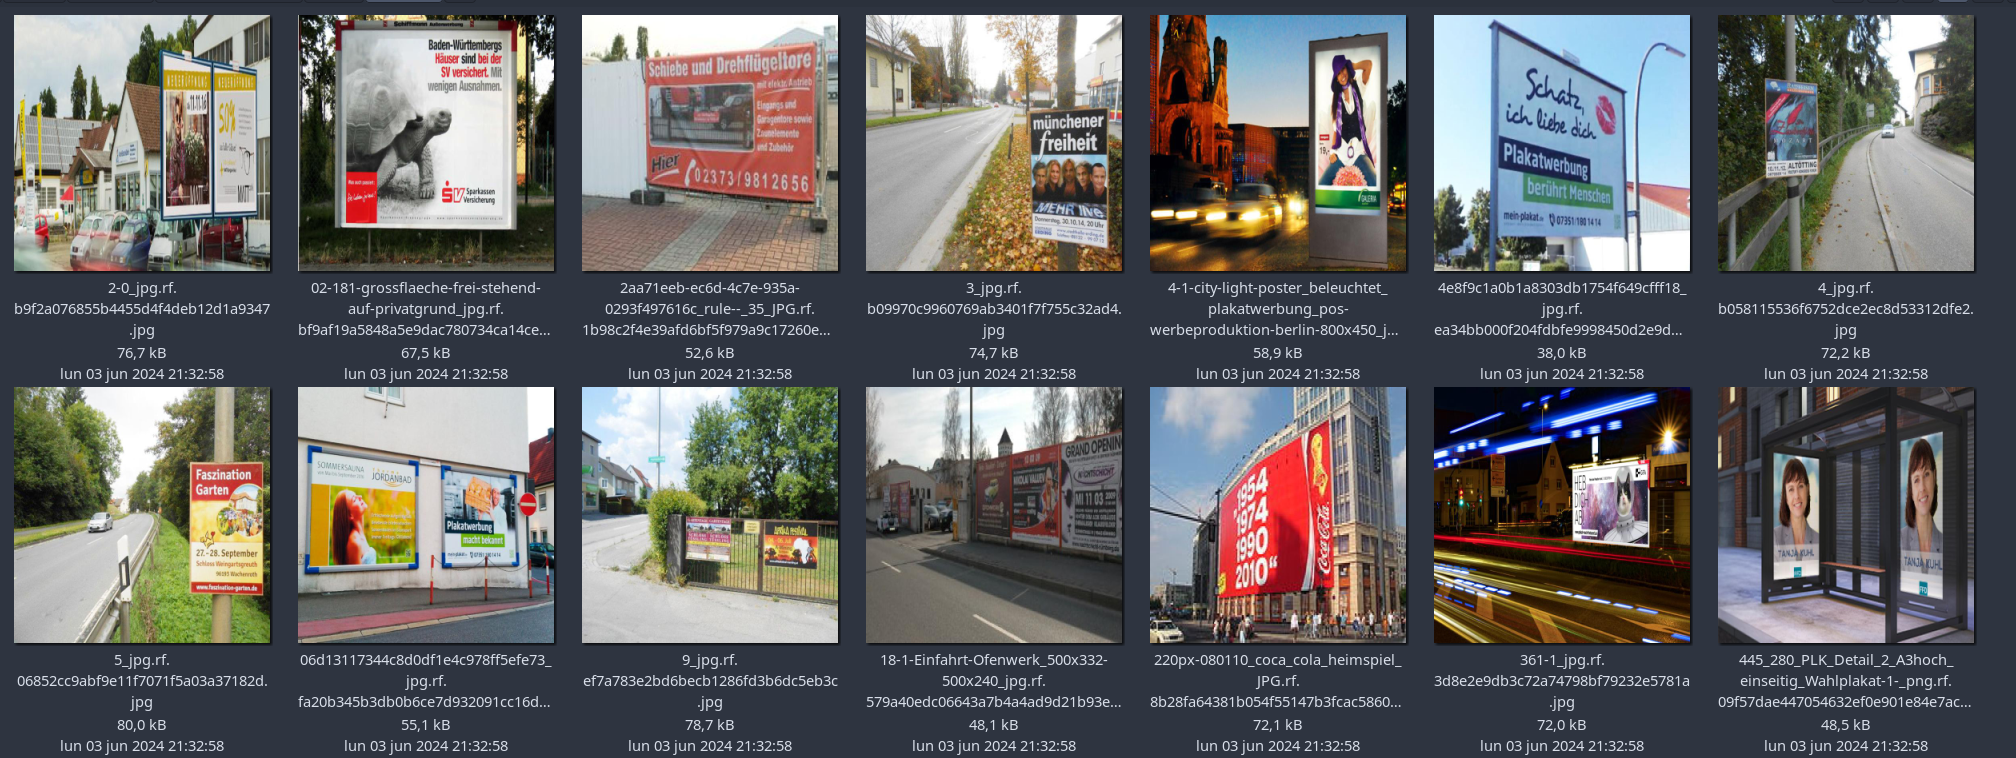
\includegraphics[width=1.1\textwidth]{./img/dataset.png}}
\caption{Un muestreo de uno de los \textit{datasets} utilizados}
\end{figure}

Otra opción ponderada fue la de construir nuestro propio conjunto de datos: sacar fotos de carteles publicitarios nosotros mismos y delimitar los rectángulos minimales manualmente para lograr tener un conjunto de datos que sabemos que son orgánicos y aún más ajustados al proyecto. Buscando minimizar los sesgos que nosotros introduciríamos (nuestras fotos serían solamente de un conjunto de calles cercanas a nosotros, siempre tomadas con los mismos dispositivos, probablemente con ángulos parecidos, etc.) y sabiendo que se requiere una magnitud considerable para la experimentación en el entrenamiento (por lo que sería un trabajo que abarcaría mucho tiempo), esta idea fue tenida en cuenta solamente en caso de no encontrar \textit{datasets} abiertos de buena calidad. \\

Además de combinar todos los \textit{datasets} que encontramos para obtener un gran volumen de datos, decidimos aplicar dos técnicas conocidas para mejorar la calidad de nuestros datos. Por un lado agregamos lo que se denominan \textit{Negative Images}: fotos donde no se encuentra ningún objeto a detectar. Esto busca que el modelo entienda que no siempre va a haber un cartel publicitario para detectar, por lo tanto debería bajar el número de predicciones categorizadas como falsos positivos (detectar un cartel donde no lo hay). Para lograr esto utilizamos el dataset de \textit{COCO} \cite{coco}, un conjunto de imágenes ya previamente clasificadas, donde filtramos imágenes de la vía pública que no tuvieran carteles, pero sí contengan personas, autos o bicicletas.

Por otro lado, aplicamos otra técnica para incrementar el volumen de nuestros datos denominada \textit{Data Augmentation}: artificialmente generar nuevas imágenes de entrenamiento, transformando las originales. Aplicando transformaciones aleatorias pero que reflejan situaciones reales, uno puede rotar, re-escalar, invertir y recortar imágenes que ya tiene en su conjunto para así influir al modelo a adaptarse mejor a situaciones desfavorables donde la cámara puede estar rotada, el cartel puede verse por la mitad o simplemente tener una imagen de peor calidad.

\subsubsection{Resultados}

Una vez determinadas las métricas para comparar modelos y un flujo para entrenarlos, fue necesario encontrar la mejor forma de comparar los distintos experimentos. Para esto utilizamos \textit{Comet} \cite{comet}, una herramienta de análisis de resultados de entrenamiento de modelos de \textit{Machine Learning}.

\textit{Comet} nos permitió centralizar el resultado de todos los entrenamientos y poder observar fácilmente la comparación entre las métricas de precisión ya mencionadas. Esto nos ayudó a decidir qué modelos descartar y qué modelos disponibilizar a través de la aplicación web.

Al finalizar la búsqueda de datasets, la exploración de hiperparámetros y optimizar el proceso de entrenamiento, llegamos al armado de seis distintos modelos, todos basados en distintos datasets, los cuales debemos analizar frente a los atributos que priorizamos al comienzo del proceso.

\begin{figure}[H]
\makebox[\textwidth][c]{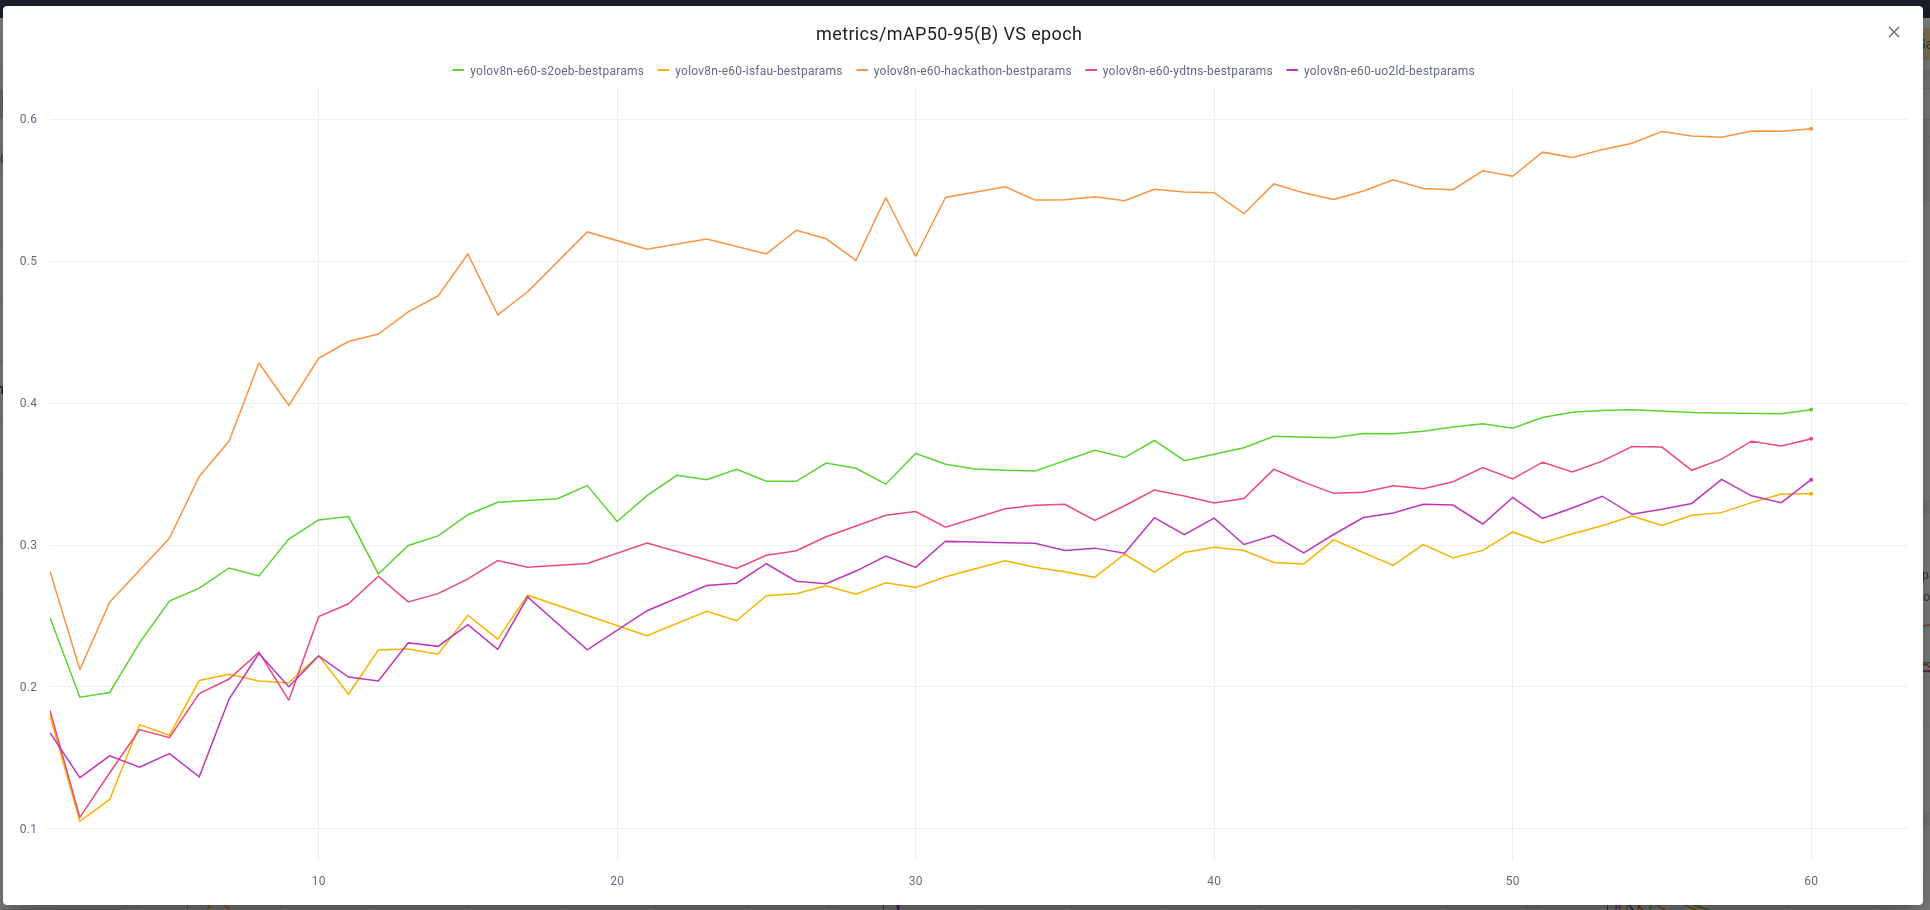
\includegraphics[width=1.1\textwidth]{./img/comet-map.png}}
\caption{Una comparación en \textit{Comet} de distintos valores de \textit{mAP50-95} para algunos de nuestros modelos finales}
\end{figure}

En resumen, la velocidad de un modelo recae principalmente sobre la arquitectura de la red, mientras que la precisión es lo que se refina con el entrenamiento.

En cuanto a la velocidad, optamos por utilizar modelos del tamaño \textit{nano}, esto es ya que no hay diferencias significativas en la precisión de modelos de distinto tamaño, pero sí en la velocidad.

\begin{table}[H]
\centering
\renewcommand{\arraystretch}{1.3}
\begin{tabular}{c c c c}
 \hline
 Modelo & Tamaño & \textit{mAP50} & Tiempo por cuadro \\
 \hline\hline
 \texttt{yolov8n-oiv7} & \textit{nano}   & 0.855 & 0.15s \\ \hline
 \texttt{yolov8s-oiv7} & \textit{small}  & 0.865 & 0.35s \\ \hline
 \texttt{yolov8m-oiv7} & \textit{medium} & 0.875 & 0.75s \\ \hline
 \texttt{yolov8l-oiv7} & \textit{large}  & 0.873 & 1.50s \\ \hline
 \texttt{yolov8x-oiv7} & \textit{xlarge} & 0.878 & 1.80s \\ \hline
\end{tabular}
\caption{Comparación de velocidad de modelos entrenados sobre \textit{Open Images} según los distintos tamaños}
\end{table}

En cuanto a la precisión, siempre basándonos en el modelo \textit{nano}, dejamos los 6 modelos y sus resultados para que el usuario pueda seleccionar cuál quiere utilizar, dejando por defecto el modelo que nosotros consideramos el mejor en base a su resultado de \textit{mAP50}.

\begin{table}[H]
\renewcommand{\arraystretch}{1.2}
\makebox[\textwidth][c]{
    \begin{tabular}{c c c c c}
    \hline
    Modelo & \# Imágenes de Entrenamiento & \textit{mAP50} & \textit{mAP50-95} \\
    \hline\hline
    \texttt{yolov8n-e60-s2oeb-bestparams}     & 8155 & 0.636 & 0.412 \\ \hline
    \texttt{yolov8n-e60-ydtns-bestparams}     & 2719 & 0.626 & 0.390 \\ \hline
    \texttt{yolov8n-e60-isfau-bestparams}     & 7137 & 0.602 & 0.360 \\ \hline
    \texttt{yolov8n-e60-uo2ld-bestparams}     & 1903 & 0.597 & 0.364 \\ \hline
    \texttt{yolov8n-e200-multi-bestparams}    & 2514 & 0.540 & 0.340 \\ \hline
    \texttt{yolov8n-e60-hackathon-bestparams} & 4503 & 0.496 & 0.315 \\ \hline
    \end{tabular}
}
\caption{Comparación de precisión de los modelos finales}
\end{table}

\subsection{Inferencia}

\subsubsection{Ejecución}

Además de existir múltiples formas de construir y entrenar un modelo, también existen múltiples formas de ejecutarlos, creando un problema de interoperabilidad donde el formato de salida del entrenamiento puede no coincidir con el formato de entrada de la inferencia.

Buscando una interfaz unificada entre estos dos polos, llegamos a \textit{ONNX}, \textit{The Open Neural Network Exchange} \cite{onnx}, ecosistema que busca estandarizar y unificar la ejecución de los modelos \textit{Machine Learning} para poder fácilmente moverse entre distintas plataformas durante todo el proceso. \\

Inicialmente, la herramienta utilizada para la lectura de los modelos fue \textit{OpenCV}, una de las principales bibliotecas de nuestro sistema que utilizamos para la preparación de los cuadros y la transformación de estos. Si bien \textit{OpenCV} es compatible con el formato \textit{ONNX}, no tiene las mejoras necesarias para tener un rendimiento optimo. La herramienta final que utilizamos en la etapa de inferencia es \textit{ONNX Runtime} \cite{ort}, cuya lectura de modelos en formato \textit{ONNX} tiene más madurez que la de \textit{OpenCV} y tiene múltiples optimizaciones aplicadas para poder proveer una ejecución más veloz del modelo.

\begin{figure}[H]
\makebox[\textwidth][c]{
    \subfloat[\centering Usando \textit{OpenCV} como el \textit{runtime} de inferencia, se promedia el procesamiento en 0.3 segundos por cuadro]{{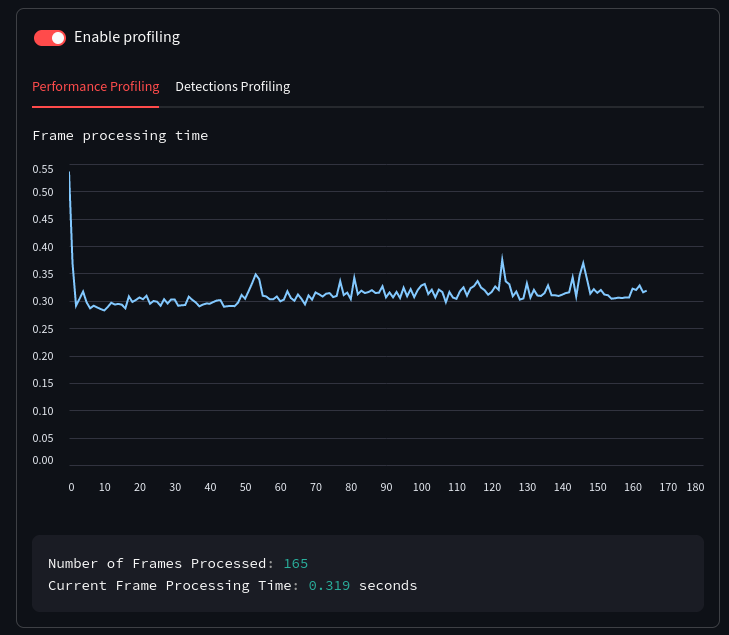
\includegraphics[width=0.55\textwidth]{./img/opencv.png} }}
    \qquad
    \subfloat[\centering \textit{ONNX Runtime} puede darnos un rendimiento de 0.15 segundos por cuadro con pocas modificaciones]{{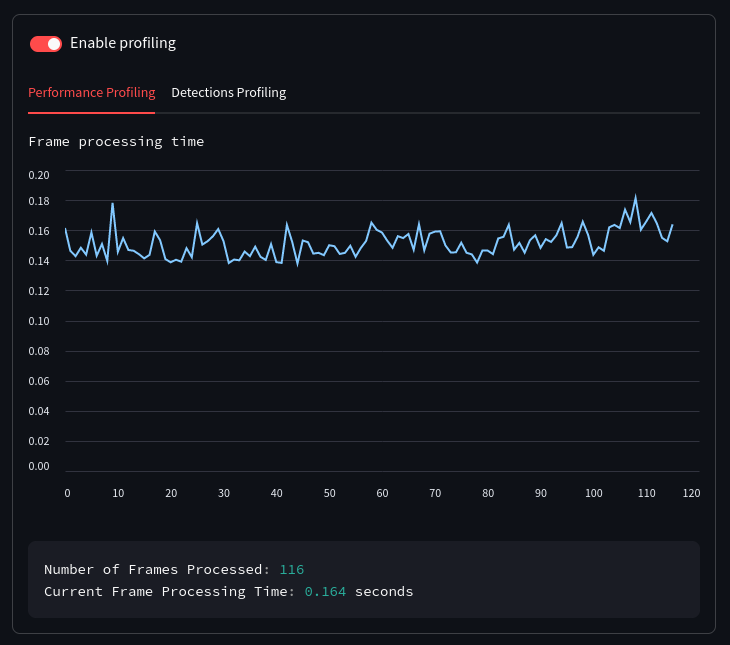
\includegraphics[width=0.55\textwidth]{./img/ort.png} }}
}
\end{figure}

Por otro lado, además de la herramienta utilizada, es importante entender que el modelo corre sobre el \textit{hardware} computacional del dispositivo que lo ejecuta. En nuestro caso, esto sucede en el servidor desplegado (ya que es este quien recibe los cuadros sobre los cuales inferir). Si bien el rendimiento óptimo de los modelos hoy en día se hace en placas de video especialmente dedicadas (\textit{GPUs}), estas representan un costo considerable el cual se puede omitir de lograr una ejecución aceptable en los procesadores (\textit{CPUs}).

Haciendo una evaluación de nuestro servidor con múltiples \textit{CPUs} de distinto tamaño de memoria, se llega a tener el rendimiento deseado sin afectar al costo del despliegue.

\begin{figure}[H]
\makebox[\textwidth][c]{
    \subfloat[\centering Un procesador de 1\textit{GB} promedia el procesamiento de cuadros en 0.2 segundos por cuadro]{{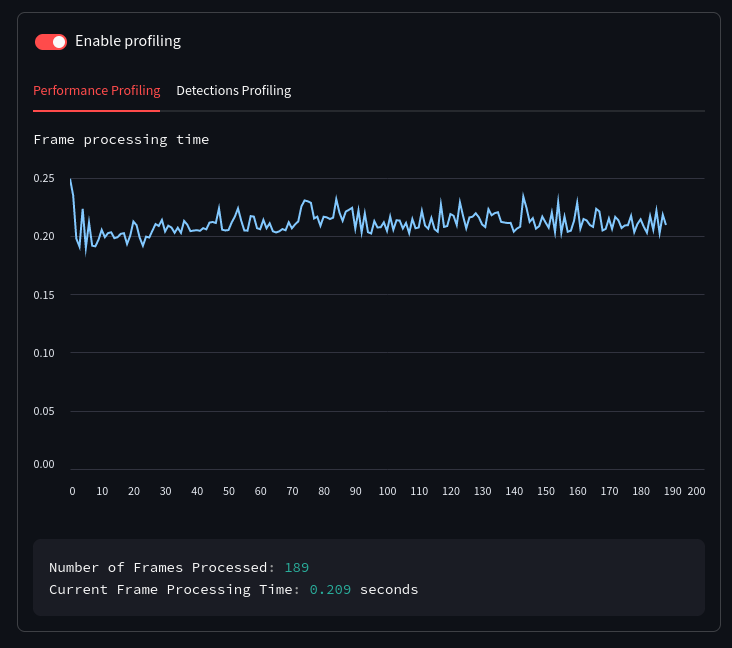
\includegraphics[width=0.55\textwidth]{./img/ort-1gb.png} }}
    \qquad
    \subfloat[\centering Un procesador de 16\textit{GB} redujo el procesamiento a la mitad, promediando en 0.1 segundos por cuadro]{{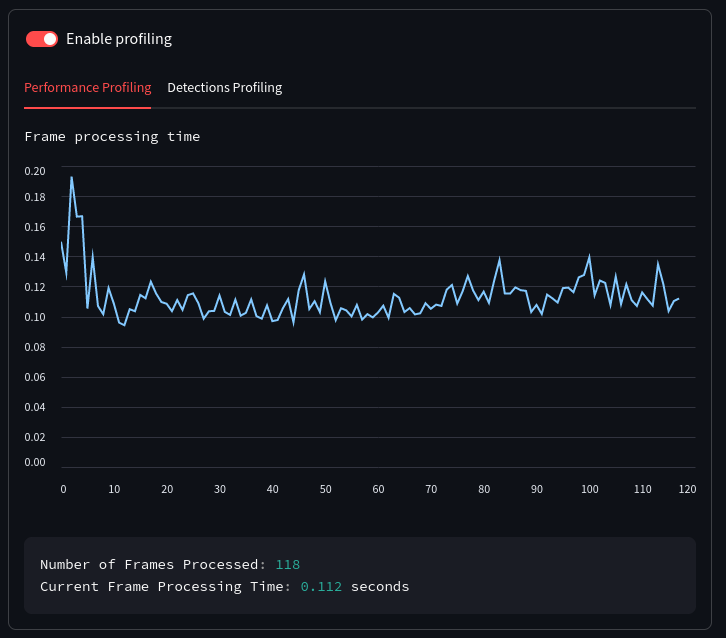
\includegraphics[width=0.55\textwidth]{./img/ort-16gb.png} }}
}
\end{figure}

\subsubsection{Transformaciones}

Una de las funcionalidades que provee nuestro sistema es la de poder elegir cómo manipular la imagen de salida del cuadro sobre el cual se hacen las detecciones, buscando que cada una cumpla un caso de uso distinto y que en un futuro sea sencillo agregar más transformaciones de así desearlo.

La transformación más sencilla que se puede aplicar sobre una imagen es la de la detección. Esta transformación consiste en solamente indicar en la imagen el rectángulo en el que se detectó que hay un objeto presente.

\begin{figure}[H]
\makebox[\textwidth][c]{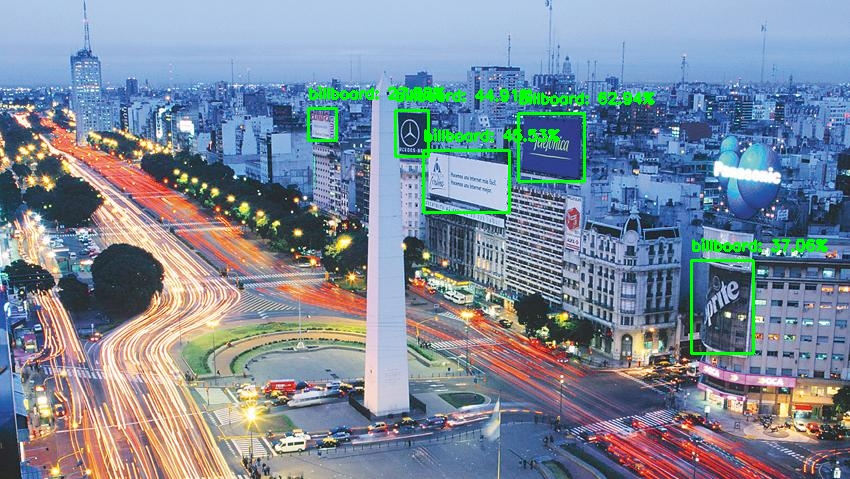
\includegraphics[width=0.9\textwidth]{./img/detect-bart.jpg}}
\caption{Detección de múltiples objetos en la misma fotografía}
\end{figure}

La segunda transformación aplicada, ya pensando en el sistema de detección de publicidades, es el \textit{blurring}. El difuminado de las publicidades sirve el propósito de indicar explícitamente que allí hay un anuncio no deseado.

\begin{figure}[H]
\makebox[\textwidth][c]{
    \subfloat{{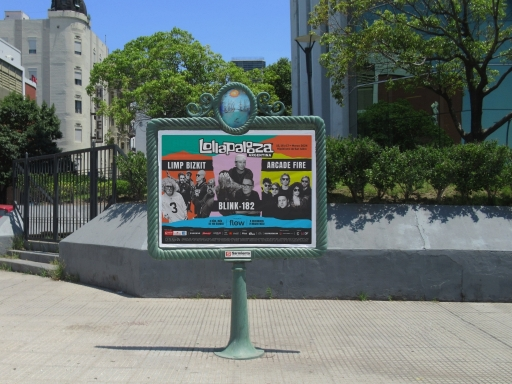
\includegraphics[width=0.5\textwidth]{./img/test.jpeg} }}
    \qquad
    \subfloat{{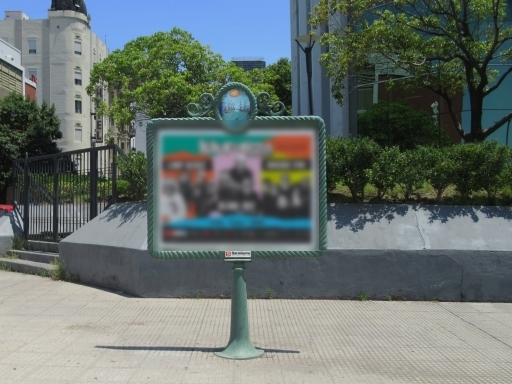
\includegraphics[width=0.5\textwidth]{./img/blur-bart.jpg} }}
}
\caption{Difuminado de objetos}
\end{figure}

La última transformación desarrollada, probablemente la más interesante de las tres, es la técnica de \textit{Image Inpainting}. Partiendo de cuando se quiere directamente remover un cartel de una imagen, buscamos qué problemas y soluciones existen en el campo de \textit{Computer Vision} para este tipo de casos. \textit{Image Inpainting} es una técnica pensada específicamente para la restauración de fotos analógicas o cuadros incompletos, donde se tienen impurezas (roturas, rayones, etc.) que se quieren reconstruir en base a sus alrededores. Esto se puede hacer de manera determinística, con un algoritmo que analiza los colores de los pixeles cercanos al hueco a rellenar, o se puede tener una red neuronal específicamente entrenada con este propósito en mente.

\begin{figure}[H]
\makebox[\textwidth][c]{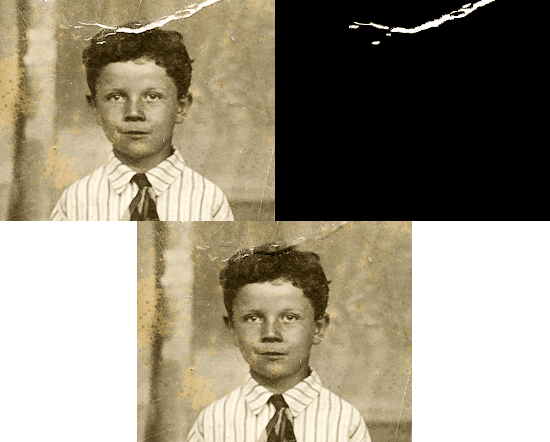
\includegraphics[width=0.5\textwidth]{./img/inpaint-old-photo.png}}
\caption{El caso de uso más tradicional de \textit{Image Inpainting} es la restauración de fotos analógicas}
\end{figure}

Si bien esta técnica no está pensada para nuestro caso de uso, donde los carteles son rectángulos que ocupan gran parte de la imagen en vez de solamente una línea o un pequeño detalle, nos pareció una buena prueba de concepto para aplicar sobre nuestro sistema y en algunos casos da resultados bastante positivos.

\begin{figure}[H]
\makebox[\textwidth][c]{
    \subfloat{{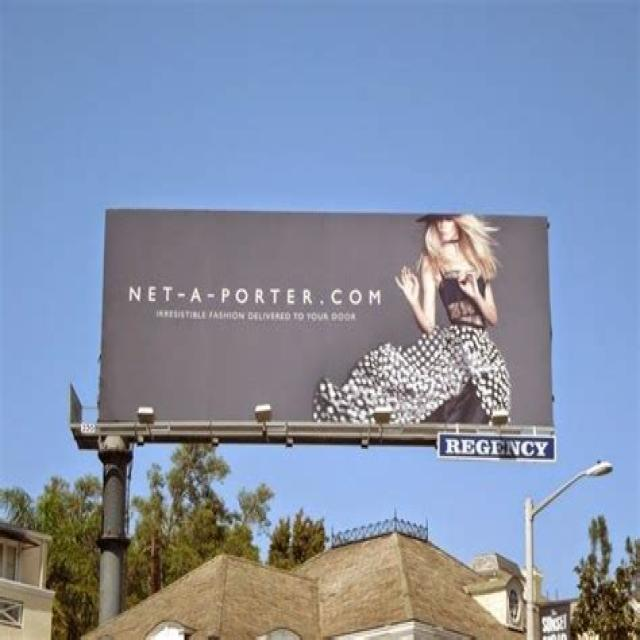
\includegraphics[width=0.5\textwidth]{./img/test-no-inpaint.jpg} }}
    \qquad
    \subfloat{{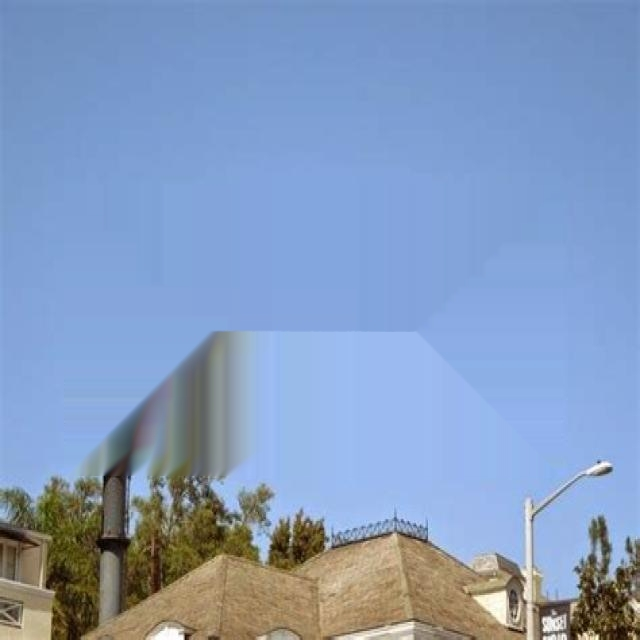
\includegraphics[width=0.5\textwidth]{./img/test-inpaint.jpg} }}
}
\caption{Eliminación de objetos a través de \textit{Image Inpainting}}
\end{figure}

\subsubsection{Optimizaciones}

Si bien dijimos que los dos atributos a priorizar en el armado de un modelo son la velocidad y la precisión, esto se puede extender a considerar el sistema en su totalidad. Más allá de que el modelo sea veloz y preciso, queremos traducir esto a la experiencia final del usuario.

Estos atributos de calidad están intrínsecamente relacionados a los videos de entrada que consume el sistema. En el traspaso de las imágenes capturadas en la cámara del usuario a la entrada del modelo, se puede manipular esta información para optimizar los atributos mencionados, nuevamente teniendo que buscar un balance entre ellos. \\

Los dispositivos de filmación pueden tomar videos en distintos \textit{frame rates} (cuadros capturados por segundo). Un video donde el frame rate sea alto, como por ejemplo de 120 cuadros por segundo, se verá más fluido que uno de menor frame rate, pero, al tener más imágenes, naturalmente será más costoso de procesar.

Una optimización que se puede aplicar en el consumo de los cuadros es decidir eliminar cuadros intermedios y pasarle menos imágenes a procesar al modelo. Al tener menos cuadros para procesar podemos mejorar la velocidad total de la inferencia del modelo, pero siempre cuidando la velocidad percibida del sistema: si se eliminan cuadros intermedios excesivamente, el video resultante será muy entrecortado y la experiencia del usuario se verá perjudicada.

Además de la cantidad de cuadros nos importa la calidad de ellos. A mayor resolución, una imagen tiene más píxeles y es más nítida, dándole más información al modelo para detectar objetos sobre ella y así tener detecciones más precisas. Pero esto también resulta en un aumento del costo de procesamiento ya que hay más información de entrada. Modificando la calidad de las imágenes a procesar podemos nuevamente balancear el intercambio entre velocidad y precisión. \\

En particular, \textit{WebRTC} nos provee de mecanismos para ajustar dinámicamente los cuadros por segundo y la calidad de estos frente a una mala conexión del cliente. Esto nos permite mantener una sesión fluida sin interrumpir el sistema y recuperar la calidad de la inferencia al obtener una mejor comunicación entre el cliente y el servidor, siempre proveyendo la mejor experiencia posible frente a las condiciones dadas.

\subsection{Presentación}

\subsubsection{Sitio Web}

La plataforma sobre la cual construimos el sitio web es \textit{Streamlit} \cite{streamlit}. Este \textit{framework} tiene el propósito de convertir \textit{software} desarrollado en \textit{Python} en páginas web que sean fácilmente compartibles, con un foco en el campo de \textit{Data Science}.

Decidimos utilizar este \textit{software} por su integración con todos los componentes que requiere nuestro sistema: tiene fácil acceso a la cámara del usuario, se integra con \textit{WebRTC} y nos da la posibilidad de desarrollar en \textit{Python}.

En particular hacemos uso del componente externo \texttt{streamlit-webrtc} \cite{streamlit-webrtc}, un componente web que facilita el uso de \textit{WebRTC} en el sitio, permitiéndonos manipular las imágenes de entrada y salida que se le presentan al usuario, así permitiéndonos preparar lo capturado por el usuario para que sea consumido por nuestro modelo, y transformar los resultados del modelo para presentarlos.

\subsubsection{Comunicación}

El protocolo de comunicación utilizado en nuestro sistema es \textit{WebRTC}, el cual se basa en coordinar conexiones \textit{peer-to-peer} entre dos dispositivos (en nuestro caso, de nuestro servidor al explorador web del usuario). Como no se puede establecer una conexión directa entre dos pares sino se sabe siquiera dónde residen, para poder establecer estas conexiones \textit{WebRTC} requiere de servidores externos que se encargan del descubrimiento (\textit{discovery}) de los pares, que se denominan \textit{STUN} y \textit{TURN}.

\begin{figure}[H]
\makebox[\textwidth][c]{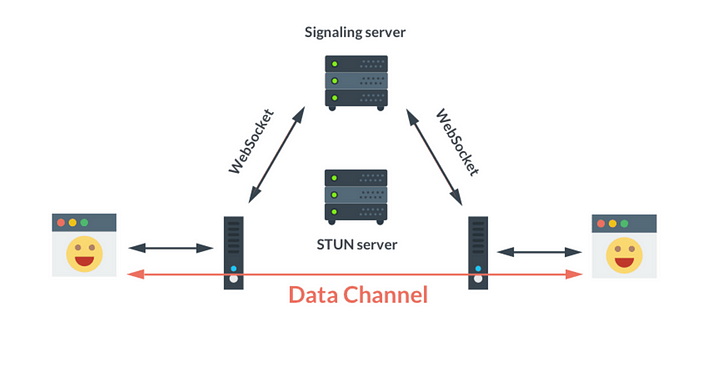
\includegraphics[width=0.8\textwidth]{./img/webrtc.png}}
\caption{\textit{WebRTC} hace uso de servidores \textit{STUN} y \textit{TURN} para establecer las conexiones par-a-par a través de \textit{WebSockets}}
\end{figure}

Hay distintos servicios que proveen servidores de este tipo que varían en calidad y no siempre funcionan en todo tipo de entornos. Después de varias evaluaciones, donde se debe procurar que el servicio ande tanto en \textit{WiFi} como en redes móviles, utilizamos el servicio provisto por \textit{Open Relay} \cite{openrelay}.

\section{Desarrollo del Trabajo}

Habiendo notado en la propuesta original del trabajo, previamente a comenzar el desarrollo, que hay una partición lógica de distintos módulos independientes, planteamos distintas metas relacionadas a cada uno de estos módulos.

\subsection{Módulos y Metas}

Los módulos en los que dividimos el trabajo al comenzar fueron:

\begin{itemize}
    \item \textbf{CV:} El objetivo de este módulo era partir de una red convolucional no propia, asumiendo que se reemplazaría en el futuro por la nuestra, y desarrollar metas relacionadas al trabajo de \textit{Computer Vision}.

    \item \textbf{CNN:} Este módulo plantea como objetivo el entrenamiento de un modelo propio  para luego poder integrar lo realizado en \textbf{CV}.

    \item \textbf{WEB:} Para el último módulo propusimos como objetivo lograr el despliegue del sistema en la web, accediendo a la cámara del cliente en tiempo real.
\end{itemize}

Estos módulos fueron desglosados en las siguientes metas parciales:

\begin{center}
\begin{tabular}{c m{0.85\linewidth}} \toprule
    \textbf{CV1} & Clasificar una imagen de acuerdo a si contiene o no contiene un cartel publicitario con una \textit{CNN} de base. \\ \midrule
    \textbf{CV2} & Evaluar los frameworks de detección de objetos como \textit{SSD}, \textit{YOLO} y \textit{R-CNN}. \newline Detectar la porción de la imagen donde se contiene el cartel. \\ \midrule
    \textbf{CV3} & Descomponer un video en sus imágenes por segundo y procesar cada una de manera separada. \\ \midrule
    \textbf{CV4} & Evaluar las implementaciones de rastreo de objetos como \textit{CSRT}, \textit{KCF} y \textit{MOSSE}. \newline Detectar los objetos en algunas imágenes del video, y rastrear su movimiento, en vez de procesar cada imagen por separado. \\ \midrule
    \textbf{CV5} & Introducir modificaciones en las imágenes del video como difuminado y resaltado. \\ \midrule
    \textbf{CV6} & Optimizar la velocidad de procesamiento de video para poder procesar los videos en tiempo real y en dispositivos de bajo poder computacional. \\ \bottomrule
\end{tabular}
\end{center}

\begin{center}
\begin{tabular}{c m{0.85\linewidth}} \toprule
    \textbf{CNN1} & Obtención de datos de carteles publicitarios. \\ \midrule
    \textbf{CNN2} & Evaluar las arquitecturas de redes convolucionales como \textit{VGGNet} o \textit{MobileNet}. \newline Armar una red convolucional que detecta carteles publicitarios. \\ \midrule
    \textbf{CNN3} & Armar una red convolucional que detecta publicidades en general (por ejemplo, logos en ropa) en vez de solamente carteles. \\ \bottomrule
\end{tabular}
\end{center}

\begin{center}
\begin{tabular}{c m{0.85\linewidth}} \toprule
    \textbf{WEB1} & Evaluar ventajas y desventajas de \textit{WASM} vs. cliente-servidor y confirmar la viabilidad de la elección. \\ \midrule
    \textbf{WEB2} & Armar un sitio web local que acceda a la cámara del usuario y utilice el modelo. \\ \midrule
    \textbf{WEB3} & Desplegar el servicio web a un servidor externo y evaluar la latencia y disponibilidad. \\ \bottomrule
\end{tabular}
\end{center}

\subsection{Cronograma Final}

En base a las metas parciales que planteamos inicialmente, diseñamos un cronograma a seguir durante el desarrollo del trabajo que fue el siguiente.

\begin{itemize}
\item \textbf{Prueba de Concepto y Viabilidad}

Abarcó las siguientes metas: \textbf{CV1}, \textbf{CV2}, \textbf{CV3}, \textbf{CNN1} \\

El objetivo principal de esta etapa del trabajo fue lograr confirmar que realizar el trabajo propuesto era viable.

Una de las fases más importantes de esta etapa fue la búsqueda de \textit{datasets} de carteles publicitarios. Una vez que encontramos un volumen de imágenes de entrenamiento que consideramos suficiente, logramos estar en condiciones de confirmar que sería posible entrenar un modelo propio para la detección de anuncios.

No era cuestión de encontrar los datos para el futuro entrenamiento solamente, además necesitábamos probar que iba a ser posible detectar objetos dentro de un video y luego aplicarle las transformaciones que nos interesaban. Para esto hicimos uso de modelos ya entrenados para otros proyectos que podían detectar objetos fáciles de conseguir como rostros de personas.

Utilizamos estos modelos ya entrenados para construir una herramienta de línea de comando que nos permitió validar, con un esfuerzo mínimo de desarrollo, que iba a ser posible aplicar transformaciones sobre cuadros de un video.

Inicialmente, la herramienta comenzó como simplemente una detección de rostros dentro de una imagen. Esta devolvía el rectángulo minimal que contiene a una cara dentro de la imagen que se le indicaba por parámetro.
Luego logramos extender su funcionalidad a que detecte rostros en videos, procesando los cuadros como imágenes independientes, resultando así en un video donde en cada cuadro tendría marcado dónde se encontraba la cara en cuestión.
Una vez que logramos hacerlo para videos, el último paso que dimos fue el de transformar cada cuadro para difuminar la cara, en vez de marcarla solamente.

Estos tres pequeños hitos que logramos con la herramienta de línea de comandos, sumado al hecho de haber encontrado suficientes imágenes de anuncios como para entrenar nuestro propio modelo, nos permitió confirmar que realizar nuestro trabajo iba a ser posible, sin haber invertido tiempo de desarrollo en lograr tener un sistema ya desplegado en la web.

Además la herramienta por línea de comando también nos permitió hacer pequeñas pruebas de concepto sobre la posible velocidad del sistema, cuántos cuadros de video podríamos omitir en la detección sin afectar sustancialmente el resultado final, cómo afectaba la calidad de la imagen a la velocidad de detección, etc. El resultado logrado en esta fase fue procesar un video en menor tiempo que su duración final (por ejemplo, procesar en 20 segundos un video de 30 segundos), así mostrando que las detecciones necesarias podrían realizarse en tiempo real o cercano a tiempo real. De todas maneras, estas pruebas son únicamente válidas para el procesamiento de un video pre-grabado, y en su eventual despliegue a un entorno de filmación constante deben ser hechas nuevamente.

\item \textbf{Arquitectura del Sistema}

Abarcó las siguientes metas: \textbf{WEB1}, \textbf{WEB2} \\

Durante esta etapa del trabajo buscamos evaluar las dos arquitecturas posibles para nuestra aplicación, cliente-servidor o detección en el cliente.

Para este punto del trabajo todavía no contábamos con nuestro modelo propio, sino que seguimos haciendo uso de los modelos públicos de detección de rostros. Esto nos permitió seguir probando las distintas alternativas y caminos que nuestro trabajo podía tomar sin siquiera invertir tiempo en entrenar un modelo propio, que sería una de las tareas que más tiempo llevaría.

Como mencionamos previamente en este trabajo, comenzamos evaluando la posibilidad de procesar la detección del modelo enteramente en el cliente, utilizando \textit{WASM}, pero finalmente por cuestiones de rendimiento de la ejecución del entorno \textit{Python} en el dispositivo optamos por utilizar una arquitectura cliente-servidor.

Una vez decidida la arquitectura construimos un sitio web (no desplegado), utilizando el framework \textit{Streamlit}, que detecta rostros de personas.

\item \textbf{Funcionalidades Avanzadas}

Abarcó las siguientes metas: \textbf{CV4}, \textbf{CNN2} \\

Una vez que construimos el sitio web local que detectaba y marcaba rostros en videos en tiempo real, tocaba entrenar nuestro propio modelo de detección de anuncios para luego reemplazar la detección de rostros por anuncios.

Para esto evaluamos una técnica dentro del campo de \textit{Computer Vision} llamada \textit{Object Tracking} (Rastreo de objetos). Lo que busca hacer esta técnica es, no solamente entender en qué parte de una imagen se encuentra un objeto dado, sino que trata de identificarlo unívocamente para poder rastrearlo con el paso de los distintos cuadros del video.

Es una técnica sofisticada que permite, por ejemplo, detectar en un video de un partido de fútbol, cuántos pases da cada jugador. Para contabilizar los pases de cada uno, deberíamos distinguir cada jugador del resto. Es allí donde el rastreo de objetos rinde frutos.
Por nuestra parte decidimos descartar esta alternativa; el alcance de las funcionalidades que buscábamos implementar en el trabajo no era tan sofisticado como para necesitar rastrear los anuncios en un vídeo.

Habiendo descartado utilizar el rastreo de objetos para nuestro trabajo, seguimos con la evaluación de distintas arquitecturas de redes convolucionales. Investigamos y comparamos varias arquitecturas distintas, como \textit{VGGNET}, \textit{Mobile}-Net, \textit{GoogLeNet}, etc. Finalmente, optamos por utilizar \textit{YOLO}, una arquitectura con bondades que ya describimos en este trabajo.

Una vez que nos decidimos por \textit{YOLO}, comenzamos con los primeros entrenamientos probando un conjunto de datos por vez, de manera iterativa. De a poco fuimos experimentando con distintas formas de entrenar, combinar conjuntos de datos, cambiar parámetros del modelo, utilizar distintos tamaños de red y demás experimentos ya descritos en el informe.

Un problema con el que nos encontramos rápidamente fue que las imágenes de entrenamiento tienen un tamaño no despreciable, por lo que se nos estaba haciendo tedioso y extremadamente lento versionar los conjuntos de datos usados junto al código de la aplicación en nuestro repositorio. Para solucionar este problema nos tomamos el trabajo de realizar un pequeño módulo de descarga de \textit{datasets}, que se ejecutaba previo al comienzo de entrenamiento de un modelo, asegurando que se descarguen todas las imágenes necesarias para poder lograr un entrenamiento consistente con los otros modelos.

\item \textbf{Trabajo Final}

Abarcó las siguientes metas: \textbf{WEB3}, \textbf{CV5}, \textbf{CV6} \\

La primera parte de la etapa final del trabajo fue desplegar el sitio web en un servidor que fuera accesible por internet desde cualquier dispositivo. Para esto, como ya mencionamos en el trabajo, usamos el servicio de \textit{Fly.io}. Vale aclarar que nuestro primer despliegue de la web no tenía nuestro propio modelo con detección de anuncios, sino que solamente funcionaba con el modelo que detectaba rostros.

Una vez que logramos disponibilizar la web a través un servidor, integramos nuestro propio modelo a la web y le dimos la opción al usuario final de elegir si quería utilizar la funcionalidad de detectar rostros o anuncios.

Para lograr esto introdujimos un polimorfismo de modelos que obliga a cualquier modelo que se ejecute en la aplicación a tener la misma interfaz de detección que los demás. Esto nos permitió desacoplar con mucha facilidad el agregado de nuevos modelos al funcionamiento de la aplicación web, que fue de mucha utilidad a la hora de comparar nuestros propios modelos entre sí.

Luego de tener nuestros propios modelos disponibles a través de la aplicación web, introdujimos la funcionalidad de \textit{Image Inpainting} junto a la ya disponible difuminación.

Además seguimos iterando distintos entrenamientos de modelos propios, para obtener nuevos resultados de posibles modelos a utilizar en la aplicación, agregando los que podían llegar a ser interesantes a la aplicación web.

Decidimos dejar la meta \textbf{CNN3} sobre detección de diversos tipos de anuncios fuera del alcance de este trabajo dado que la complejidad de esta tarea pasaba por seguir buscando nuevos conjuntos de datos que nos permitieran extender los modelos que ya teníamos, algo que no consideramos de extrema relevancia para el trabajo.

Finalmente, seguimos ajustando detalles sobre la aplicación web. Cambiamos el intérprete del modelo de \textit{OpenCV} por el de \textit{ONNX Runtime}, modificamos los recursos utilizados por nuestra plataforma de despliegue, agregamos nuevos modelos y cambiamos el proveedor de servidores \textit{STUN} y \textit{TURN} para \textit{WebRTC}, con el fin de mejorar la experiencia para el usuario final.

Con estos últimos ajustes finalizamos un trabajo que cumple los objetivos establecidos, logra un rendimiento deseado y proporciona las funcionalidades inicialmente planteadas, encontrando en el camino oportunidades para futuras extensiones.

\end{itemize}

\newpage
\section{Conclusiones y Trabajo Futuro}

Finalizando, notamos distintas lecciones y aprendizajes que tomamos del desarrollo del trabajo en su totalidad, y rumbos posibles que se nos ocurren para el sistema en un futuro. \\

Lo primero que podemos decir del desarrollo es que nos adentró a un campo del cual no teníamos ningún tipo de experiencia práctica y nos reveló que existen múltiples problemas abiertos por solucionar y cómo de cada idea que puede surgir ya hay un cúmulo de investigación inmenso del cual partir.
Además de la abundancia de investigación, nos sorprendió la calidad de la experiencia de desarrollo. Frente a cada problema que nos encontramos, se nos presentaron múltiples herramientas a evaluar que hicieron más fácil nuestro trabajo. Nos otorgaron soluciones tanto a bajo como a alto nivel de entendimiento del problema, según lo requiriésemos. El presente trabajo se logró gracias a las distintas herramientas que usamos y sin ellas no podría haber salido de la forma buscada. \\

\textit{Computer Vision} es un campo de alta complejidad con muchos matices y opciones para investigar, es por esto que de querer extender este trabajo y las funcionalidades del sistema desarrollado, se nos presentan múltiples ideas que se podrían tener en cuenta:

\begin{itemize}
\item \textbf{Rastreo de Objetos:} Si bien nosotros descartamos utilizarlo porque lo consideramos fuera del alcance, puede ser una herramienta muy interesante para generar nuevos tipos de estadísticas sobre el video que está siendo procesado. Por ejemplo, podríamos ofrecerle al usuario las marcas de tiempo exactas donde se vio un anuncio específico en el video, o un contador de cuántas veces aparece cada anuncio, rastreando cuándo un anuncio específico entra y sale de pantalla.


\begin{figure}[H]
\makebox[\textwidth][c]{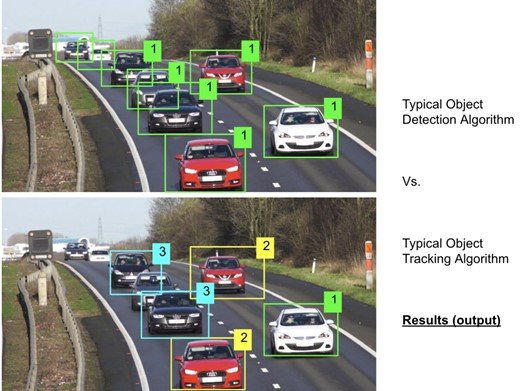
\includegraphics[width=0.7\textwidth]{./img/multiple-object-tracking.jpg}}
\caption{El \textit{Object Tracking} identifica cada objeto detectado unívocamente}
\end{figure}

\item \textbf{Segmentación:} En nuestra implementación, el difuminado del anuncio se hace marcando el centro del rectángulo que lo contiene y aplicando una difuminación gaussiana que difumina más en el centro y menos a medida que se aleja de él. Si bien es una solución aceptable, no es perfecta. Se podría mejorar reemplazando la detección del modelo con rectángulo minimal actual por los segmentos indicados con la técnica de \textit{Object Segmentation}. Esta técnica además de entender dónde está el objeto en la imagen da información sobre la forma exacta del mismo. Esto podría permitir hacer transformaciones sobre la imagen con mayor precisión.

\begin{figure}[H]
\makebox[\textwidth][c]{
    \subfloat[\centering Los distintos problemas de \textit{Computer Vision} dentro de los cuales se encuentran los tipos de segmentación]{{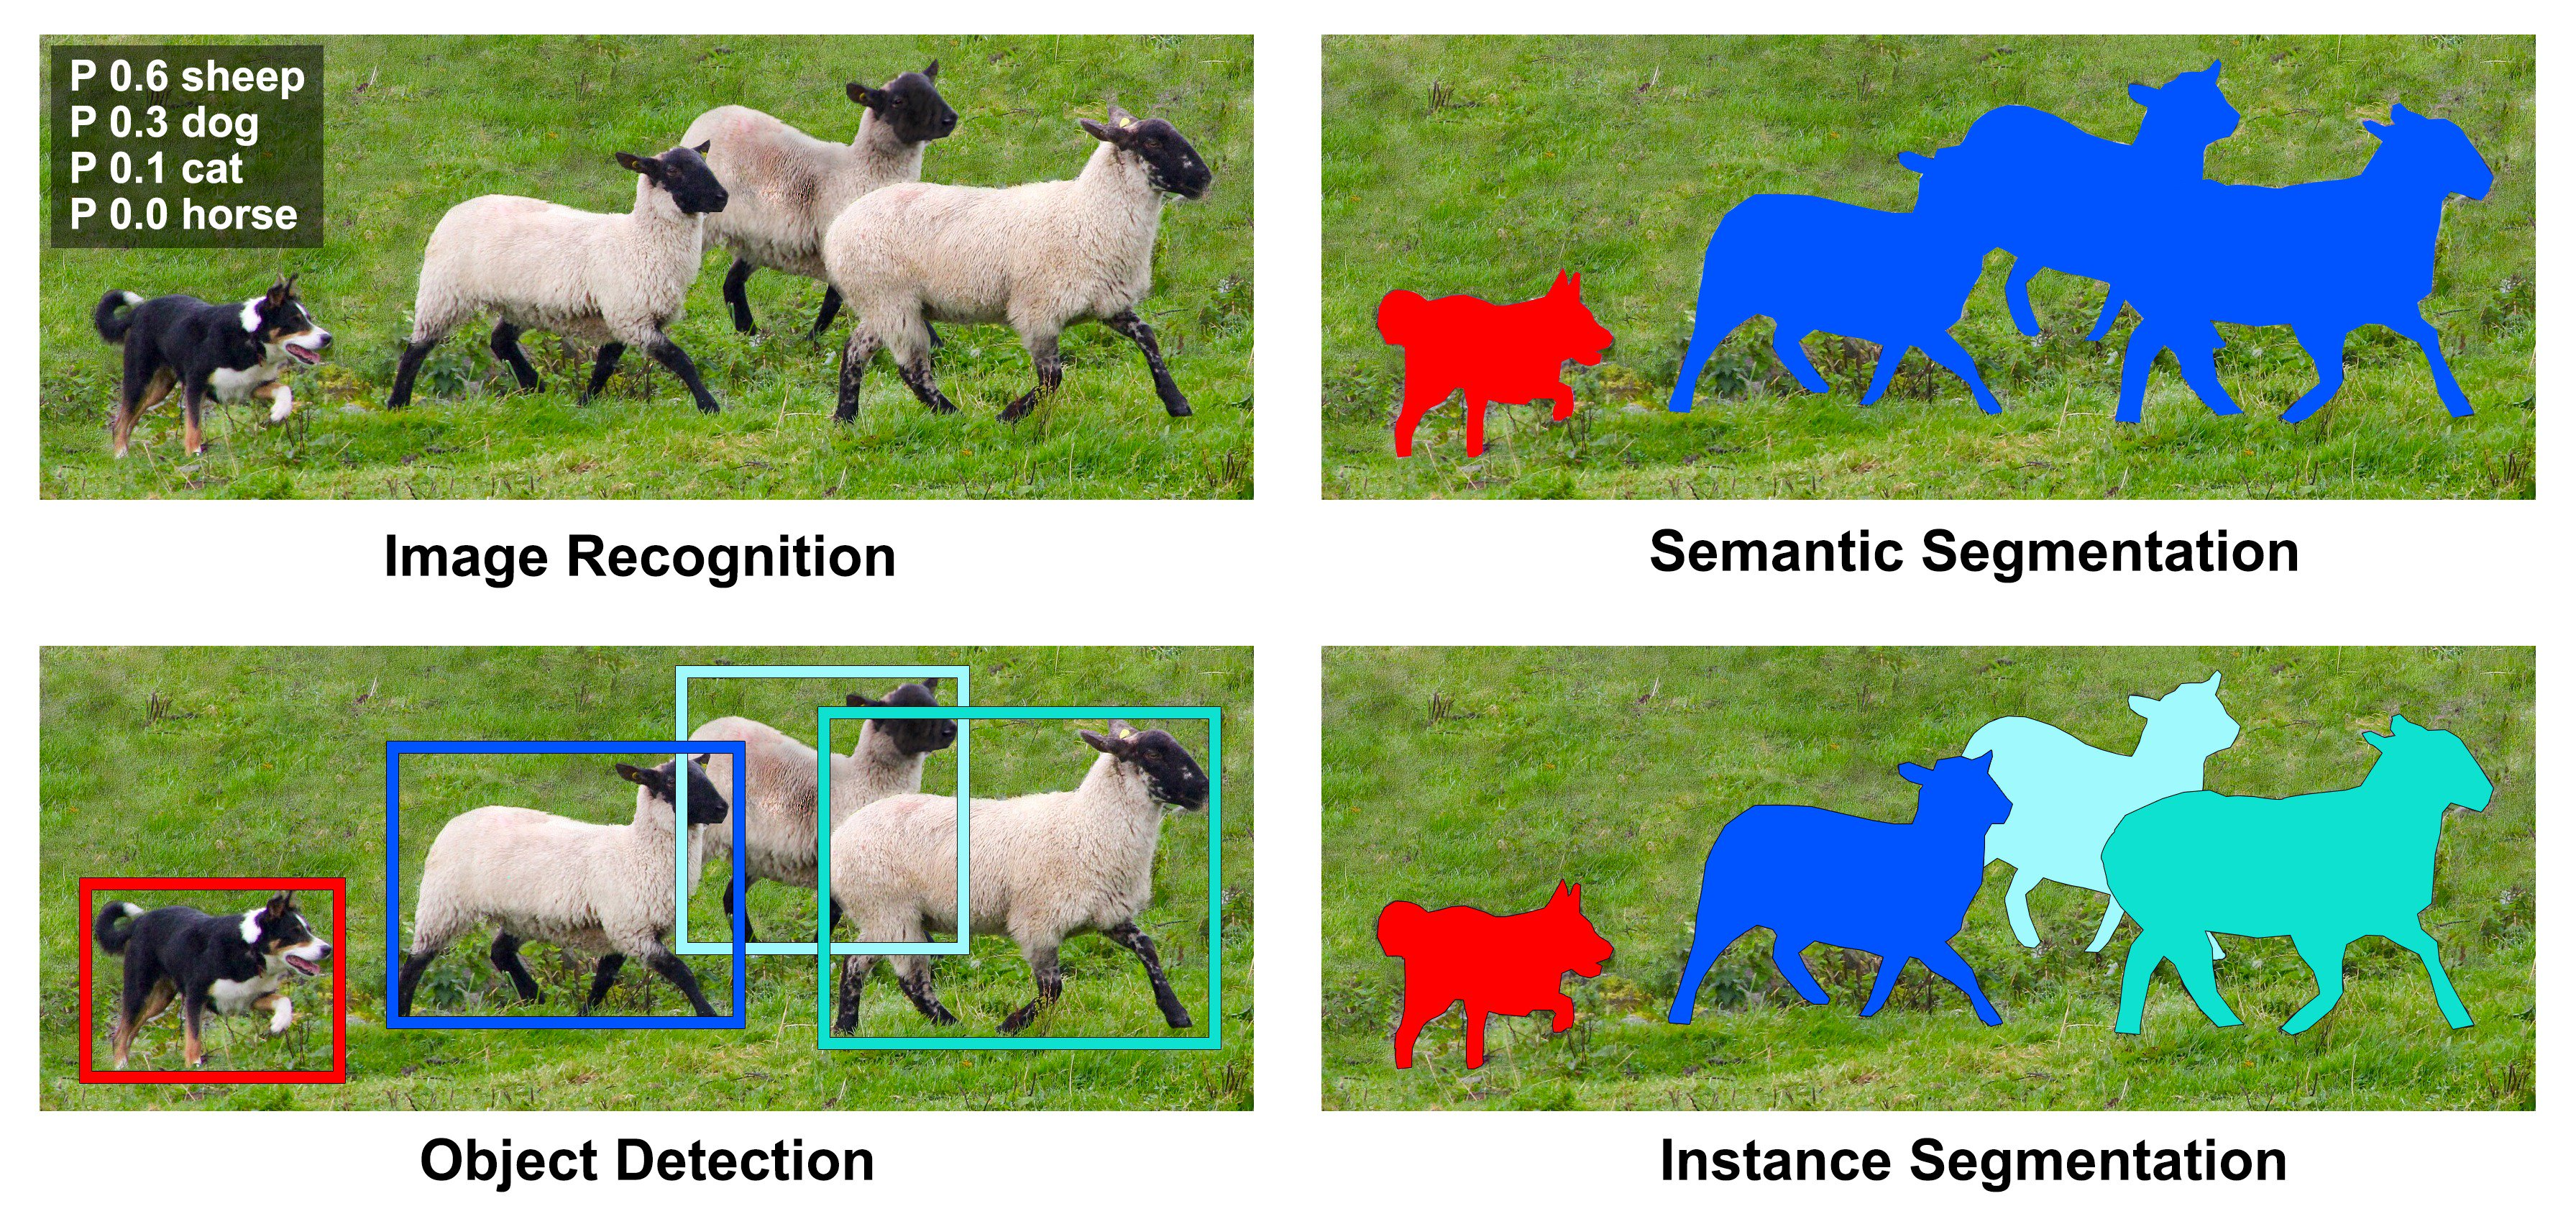
\includegraphics[width=0.75\textwidth]{./img/segmentation-goat.jpeg} }}
    \qquad
    \subfloat[\centering En nuestro caso, la segmentación se aplicaría sobre carteles publicitarios]{{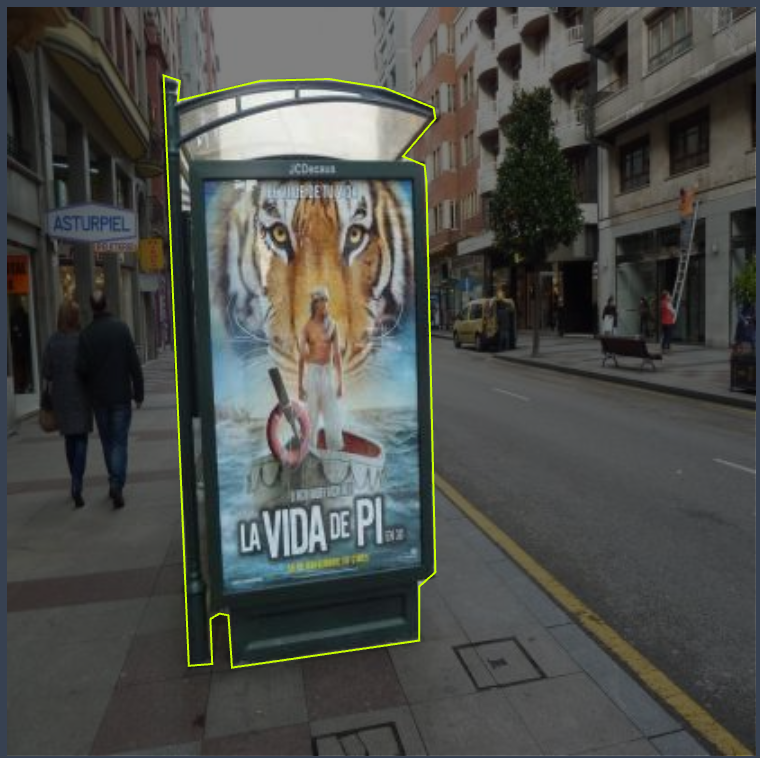
\includegraphics[width=0.35\textwidth]{./img/segmentation.png} }}
}
\end{figure}

\item \textbf{Clasificación multi-clase:} Arbitrariamente decidimos que el alcance del trabajo era para carteles de publicidad en la vía pública, pero es enteramente posible re-entrenar los modelos con otros tipos de publicidades como marcas, logos, e incluso detectar situaciones sutiles de \textit{product placement} en películas o series de televisión.

\begin{figure}[H]
\makebox[\textwidth][c]{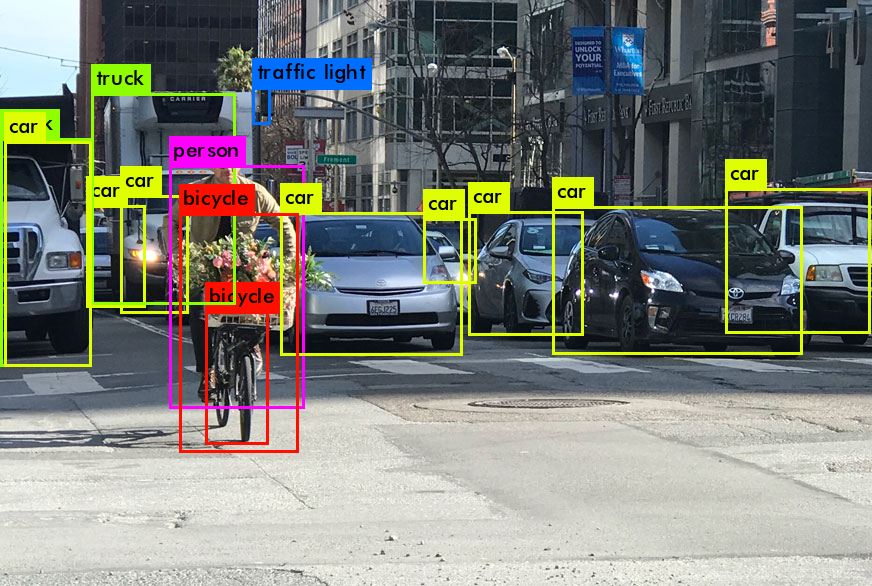
\includegraphics[width=0.6\textwidth]{./img/multi-class.png}}
\caption{La multi clasificación identifica distintas categorías de objetos en la misma imagen}
\end{figure}

\end{itemize}

Asimismo, en el transcurso del trabajo fuimos testigos de cómo este es un campo que todavía está en constante cambio y mejora. Solo por dar un ejemplo, al comenzar este trabajo la implementación más avanzada de la familia de algoritmos \textit{YOLO} era \textit{YOLOv8} (presentado en enero de 2023 \cite{yolov8}) y al finalizarlo comenzamos a ver implementaciones de \textit{YOLOv10} (publicado en mayo de 2024 \cite{yolov10}). Es claro que esta podría ser otra opción para la extensión del trabajo, uno podría partir de los mismos conjuntos de datos que ya utilizamos nosotros y recrear todos nuestros entrenamientos utilizando versiones más modernas de \textit{YOLO} para comparar las mejoras o directamente mejorar la aplicación web. \\

Es importante notar que también nos encontramos frente a una evolución constante en otros campos que dependen de \textit{Computer Vision}, siendo que la información visual sigue creciendo cada vez más como la interfaz elegida por preferencia, donde por ejemplo un modelo de lenguaje grande como \textit{GPT} introdujo recientemente la interpretación de fotografías como entrada \cite{chatgpt-vision}.

Es por esto que también podemos dejar atrás la idea de que el video siempre va a estar filmado desde un dispositivo celular y pensar en qué otras plataformas podríamos desplegar este sistema, como podría ser un casco de realidad virtual. Conociendo lo popular que es la idea de tener un \textit{software} que oculte anuncios en nuestro explorador web (un \textit{ad blocker}), no nos parece ilógico pensar que alguien quiera ocultar anuncios en la vida real mientras está usando un dispositivo como los cascos \textit{Meta Quest} o \textit{Apple Vision Pro}. \\

El entrenamiento de los modelos es un proceso muy costoso que requiere un uso intensivo de recursos. Si bien es cierto que aprovechamos las ventajas de todas las investigaciones disponibles y las herramientas de código libre y abierto para poder realizar este trabajo, no dejamos de tener que lidiar con la necesidad de precisar un alto poder computacional para lograr buenos resultados en un tiempo razonable. Hoy en día existen soluciones a esta problemática donde uno puede pagar por unidades de procesamiento gráficas modernas y potentes lo cual hace que las iteraciones de entrenamiento sean mucho más rápidas y puedan hacerse sobre mayor cantidad de datos, resultando así en un mejor resultado final. Si bien nuestro proyecto no lo requirió, esto nos muestra cómo el tener mejor \textit{hardware} ayuda a mitigar el balance entre velocidad y precisión que planteamos en el proyecto. Sabiendo que el \textit{hardware} es algo que mejora muy rápidamente con el tiempo, sería interesante revisar cómo replicar este proyecto en unos años. Además, nos muestra cómo el entrenamiento de modelos, por más que las herramientas de \textit{software} puedan ser las mismas para todos, está atado a la inversión monetaria que se haga en este, indicando que si se quiere competir efectivamente en este campo se necesitan recursos significativos. \\

En definitiva, este proyecto nos permitió aprender y aplicar técnicas avanzadas de \textit{Computer Vision}, revelándonos tanto su potencial como sus desafíos, y mostrándonos las oportunidades interesantes que van a surgir en el campo con el avance de estas tecnologías.

\newpage
\onehalfspacing

\setcounter{secnumdepth}{0}
\begin{thebibliography}{999}

\bibitem{yolov1} Redmon, Joseph, et al. (2016) \textit{You Only Look Once: Unified, Real-Time Object Detection.}
\bibitem{ultralytics} \textit{Ultralytics}: \url{https://docs.ultralytics.com/}
\bibitem{roboflow} \textit{Roboflow}: \url{https://universe.roboflow.com/}
\bibitem{opencv} \textit{OpenCV}: \url{https://opencv.org/}
\bibitem{openimages} \textit{Open Images}: \url{https://storage.googleapis.com/openimages/web/index.html}
\bibitem{wasm} \textit{WebAssembly}: \url{https://webassembly.org/}
\bibitem{pyodide} \textit{Pyodide}: \url{https://pyodide.org/}
\bibitem{webrtc} \textit{WebRTC}: \url{https://webrtc.org/}
\bibitem{flyio} \textit{Fly.io}: \url{https://fly.io/}
\bibitem{coco} \textit{COCO Dataset}: \url{https://cocodataset.org}
\bibitem{comet} \textit{Comet}: \url{https://www.comet.com/}
\bibitem{onnx} \textit{ONNX}: \url{https://onnx.ai/}
\bibitem{ort} \textit{ONNX Runtime}: \url{https://onnxruntime.ai/}
\bibitem{streamlit} \textit{Streamlit}: \url{https://streamlit.io/}
\bibitem{streamlit-webrtc} \texttt{streamlit-webrtc}: \url{https://github.com/whitphx/streamlit-webrtc}
\bibitem{openrelay} \textit{Open Relay}: \url{https://www.metered.ca/tools/openrelay/}
\bibitem{yolov8} \textit{YOLOv8}: \url{https://docs.ultralytics.com/models/yolov8/}
\bibitem{yolov10} Wang, Ao, et al. (2024) \textit{YOLOv10: Real-Time End-to-End Object Detection}
\bibitem{chatgpt-vision} \textit{GPT-4o}: \url{https://openai.com/index/hello-gpt-4o/}

\end{thebibliography}

\section{Bibliografía}

Rosebrock, Adrian. (2017). \textit{Deep learning for Computer Vision with Python.}

Ansari, Shamshad. (2020). \textit{Building Computer Vision Applications Using Artificial Neural Networks}, Apress.

Moroney, Laurence. (2020). \textit{AI and Machine Learning for Coders}, O'Reilly.

\end{document}
